\documentclass[a4paper, 11pt, oneside]{book}
\include{../../Preambles/LectureNotesPreamble}
\graphicspath{{/Complexity/}}

\begin{document}

\lfoot{\footnotesize Computational models, \\Computability and Complexity 67521}

\begin{titlepage}
    \begin{center}
        \vspace*{1cm}

        \LARGE
        \textbf{Computational models, Computability and Complexity 67521}

        \vspace{0.5cm}
        \Large
        Based on lectures by Prof. Orna Kupferman, recitations by Ms. Maya Dotan and comments by Zip and Kent 

        \vspace{1.5cm}
        \large
        \textbf{Notes by Asaf Etgar}\\
        Spring 2021\\
        

%        \vfill
%\begin{figure}[H]
%	\centering
%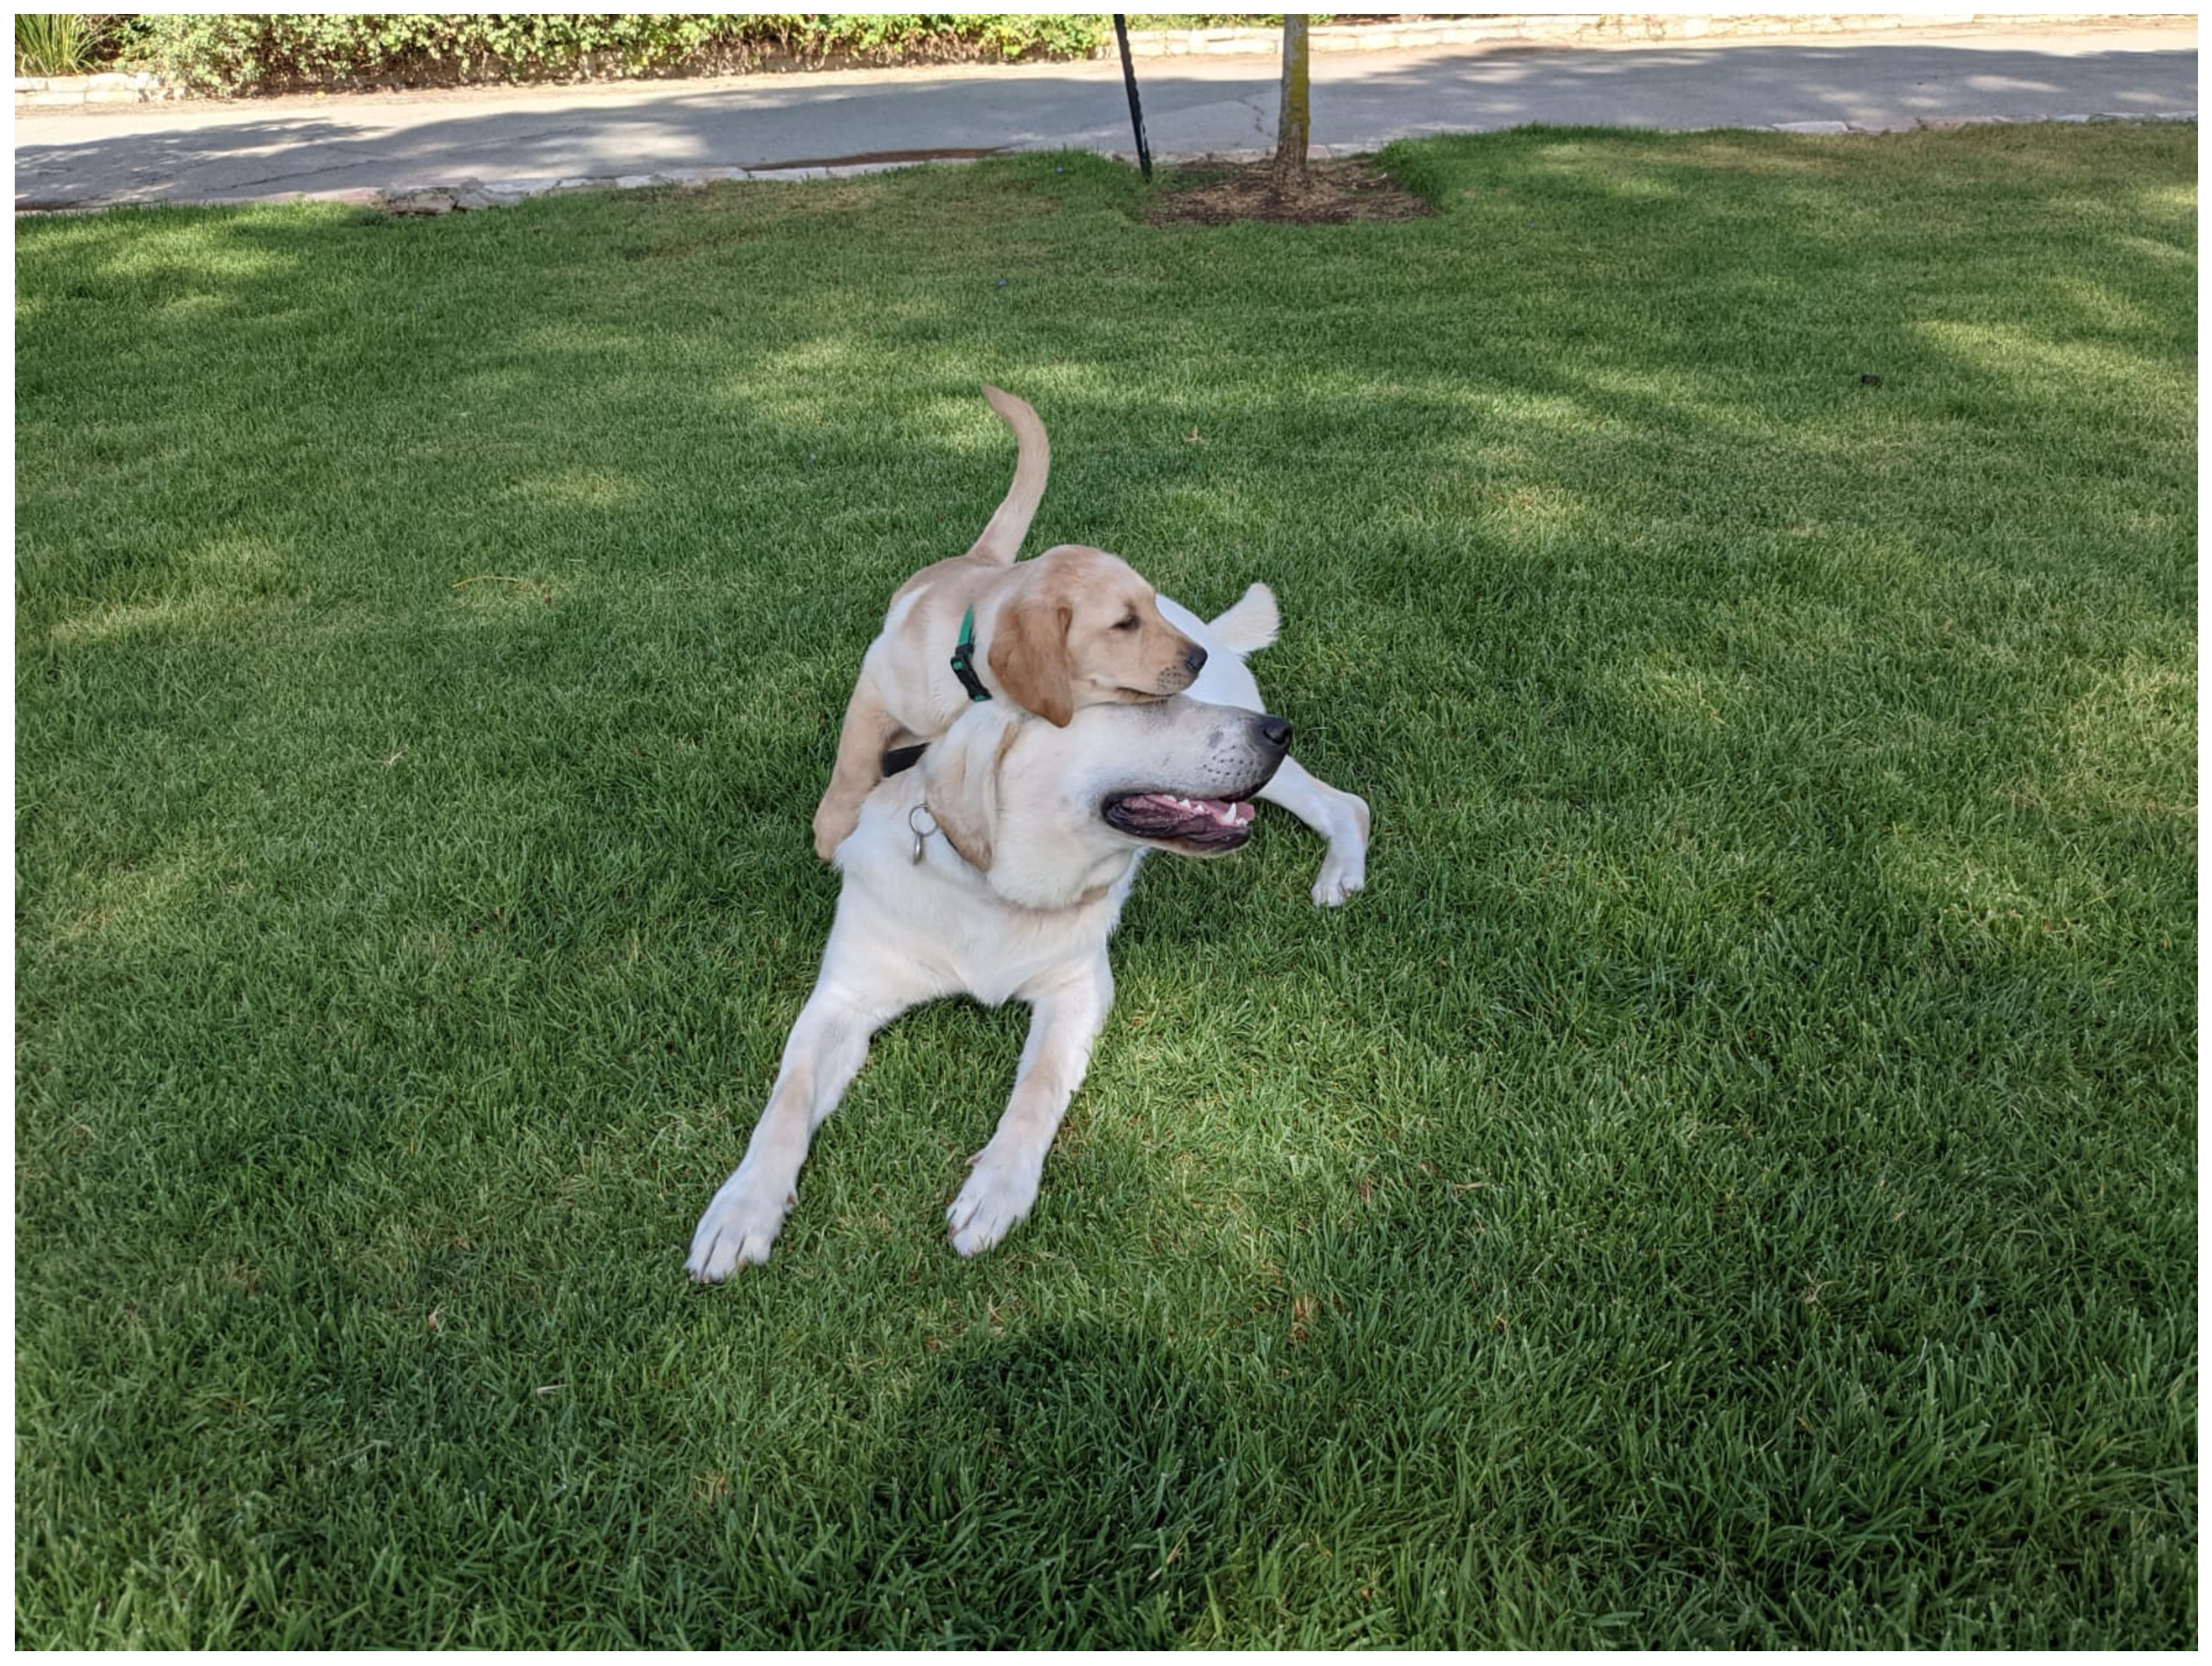
\includegraphics{zip.eps}
%\caption{"As long as he's not charging towards me" (Zip \& Kent)}
%\end{figure}



        \vspace{0.8cm}

        \large
        Last edit:
        \today \\
        For any corrections, requests for additions or notes - please email me at \\
        \ttfamily{asafetgar@gmail.com}\\
        		\vspace{0.8cm}
        \textit{These notes have not been revised by the course staff, and some things may appear differently than in the lectures/ recitation.}

    \end{center}
\end{titlepage}
\tableofcontents
\part{Automata and Languages}
\chapter{Regular languages}
A finite automata is a finite state machine, designed to formalize the idea of "legal sequences of commands". To define an automata we would need some notion of commands, and a way to describe transitions between commands - in a way that captures (in)validity of a given sequence of commands.
\section{Finite Automata}
\begin{yellowBox}
	\begin{defn}[Alphabet] An \textbf{Alphabet} denoted by $\Sigma$ is a finite set of letters $\Sigma = \{\sigma_1, \sigma_2\ldots \sigma_n\}$
	\end{defn}
\end{yellowBox}
\begin{example} Some alphabet:
	\begin{itemize}
		\item $\Sigma = \{0,1\}$
		\item $ \Sigma = \{\text{On, Off, U,D,L,R}\}$
	\end{itemize}
\end{example}
\begin{yellowBox}
	\begin{defn}[Word, Empty Word] A \textbf{Word} is a finite sequence of letters from a given alphabet. Denote the \textbf{Empty word} by $\varepsilon$. Denote the collection of all words over $\Sigma$ by $\Sigma^*$, and note that $|\Sigma^*| = \aleph_0$ when $\Sigma$ is finite.
	\end{defn}
	\begin{defn}[Language] A \textbf{Language} is a subset of words $\Ll\subset \Sigma^*$ (we do not distinguish proper and improper inclusion).
	\end{defn}
	\begin{defn}[Finite Automaton] A \textbf{Finite Automaton} consists of $5$ items: $(Q,\Sigma, \delta, q_0, F)$, with:
		\begin{itemize}
			\item $Q$ state set.
			\item $\Sigma$ alphabet.
			\item $\delta: Q\times \Sigma \To Q$ transition function.
			\item $q_0\in Q$ initial state.
			\item $F\subset Q$ subset of accepting states.
		\end{itemize}
	\end{defn}
\end{yellowBox}
\begin{example}
	Define: $\Sigma = \{0,1\}$, $Q = \{q_0, q_1\}$:
	\begin{figure}[H]
		\centering
		\begin{tikzpicture}[shorten >=1pt,node distance=3cm,on grid,auto]
			\node[state,initial] (q_0)   {$q_0$};
			\node[state] (q_1) at (2,0) {$q_1$};
			
			
			\path[-stealth, thick]
			(q_0) edge [bend left] node{0} (q_1)
			edge [loop above] node{1} (q_0)
			(q_1) edge [bend left] node{0} (q_0)
			edge [loop above] node{1} (q_1);
		\end{tikzpicture}
		\caption{Simple Automaton}
	\end{figure}
	Note that here $\delta$ is implied, and that $F = \emptyset$. We may define $F = \{q_0\}$, and get the automaton:
	\begin{figure}[ht]
		\centering
		\begin{tikzpicture}[shorten >=1pt,node distance=3cm,on grid,auto]
			\node[state,initial, accepting] (q_0)   {$q_0$};
			\node[state] (q_1) at (2,0) {$q_1$};
			
			
			\path[-stealth, thick]
			(q_0) edge [bend left] node{0} (q_1)
			edge [loop above] node{1} (q_0)
			(q_1) edge [bend left] node{0} (q_0)
			edge [loop above] node{1} (q_1);
		\end{tikzpicture}
		\caption{Simple Automaton with accepting state} 
	\end{figure}
\end{example}
\begin{yellowBox}
	
	\begin{defn}[A Run on Automaton] Let $\Aa$ be an automaton and $w = (w_i)_{i=1}^n\in \Sigma^*$ a word. A \textbf{Run} $R$ on $A$ is a sequence of states $R = (r_i)_{i=0}^{n}\in Q$ such that $r_0 = q_0$ and
		\begin{flalign*}
			\forall 0\leq i \leq n-1 \qquad r_{i+1} = \delta(r_i, w_{i+1})
		\end{flalign*}
		That is -$R$ behaves according to $\delta$ ($R$ respects $\delta$).
	\end{defn}
	\begin{defn}[Accepting Run]
		We say a run $R$ is \textbf{accepting} if $r_n\in F$
	\end{defn}
\end{yellowBox}
\begin{example}
	Recall the previous automaton with the word $1101$, we get the run $$q_0\nim{1}\to q_0\nim{1}\to q_0\nim{0}\to q_1\nim{1}\to q_1$$ Which is not accepting. Conversely -  The run on $0101$ is:
	$$q_0\nim{0}\to q_1 \nim{1}\to q_1\nim{0}\to q_0 \nim{1}\to q_0$$
	Which is accepting, because $q_0\in F$.
\end{example}
\begin{yellowBox}
	\begin{defn}[Accepting a word - deterministic] We say an automaton $\Aa$ \textbf{Accepts} a word $w$ if the (single) run $R$ on $w$ is accepting
	\end{defn}
	\begin{defn}[Language of Automaton] The \textbf{Language of Automaton} $\Aa$ is:
		$$\Ll(\Aa) = \{w \mid \Aa \text{ Accepts } w\}$$
	\end{defn}
\end{yellowBox}
\begin{example}
	For the previous automaton $\Aa$, we have $\Ll(\Aa) = \{w\mid \text{the number of $0$s in $w$ is even}\}$. Note that this is not a proof, but a claim. We will see later how to prove these claims (in various ways).
\end{example}
\begin{remark}
	Until now, we demanded that $\delta$ is defined for any $q\in Q, \sigma\in \Sigma$ (that is, $A$ is \textbf{complete}). We could ignore this demand, and assume that for an incomplete automata - we could extend the incomplete $\delta$ to a complete one by introducing a \textbf{Rejecting Sink} $q_{rej}\in Q\setminus F$ and extend $\delta$ accordingly.
\end{remark}
\begin{example} Consider the following automaton
	\begin{figure}[ht]
		\centering
		\begin{tikzpicture}[shorten >=1pt,node distance=3cm,on grid,auto]
			\node[state,initial] (q_1)   {$q_1$};
			\node[state, accepting] (q_2) at (2,0) {$q_2$};
			\node[state] (q_3) at (4,0) {$q_3$};
			
			\path[-stealth, thick]
			(q_1) edge [loop above] node{0} (q_1)
			edge [ bend left] node{1} (q_2)
			(q_2) edge[loop above] node{1} (q_2)
			edge[bend left] node{0} (q_3)
			(q_3)		edge [bend left]node{0,1} (q_2)
			;
		\end{tikzpicture}
		\caption{Example Automaton $\Aa$} 
	\end{figure}
	What is $\Ll(\Aa)$? Check a few words:
	\begin{itemize}
		\item $000$ is not accepted
		\item $00010$ is not accepted
		\item $01101$ is accepted
	\end{itemize}
	The language is $$L(A) = \{w\mid \text{There is at least one $1$, and after the last $1$ there is an even number of $0$}\}$$
\end{example}
\begin{example} Consider the following language:
	$$
	\Ll_2 = \{w\in \{0,1\}^* \mid \text{$w$ contains $001$}\}
	$$
	We design the automaton:
	
	\begin{figure}[H]
		\centering
		\begin{tikzpicture}[shorten >=1pt,node distance=3cm,on grid,auto]
			\node[state,initial] (q0)   {$q_0$};
			\node[state] (q1) at (2,0) {$q_1$};
			\node[state] (q2) at (4,0) {$q_2$};
			\node[state, accepting] (qacc) at (6,0) {$q_3$};
			
			\path[-stealth, thick]
			(q0) edge [loop above] node{1} (q0)
			edge [bend left] node{0} (q1)
			(q1) edge[bend left] node{1} (q0)
			edge [bend left] node{0} (q2)
			(q2) edge[bend left] node{1} (qacc)
			edge [loop above] node{0} (q2)
			
			(qacc) edge [loop above] node{0,1} (qacc);
		\end{tikzpicture}
		\caption{Automaton for $\Ll_2$}
	\end{figure}
	
\end{example}
\newpage
\begin{example}
	We extend the last example, define:
	$$ \Ll_n = \{w\mid \text{$w$ contains $0^n 1$}\} $$
	A fitting automaton would be:
	
	\begin{figure}[H]
		\centering
		\begin{tikzpicture}[shorten >=1pt,node distance=3cm,on grid,auto]
			\node[state,initial] (q0)   {$q_0$};
			\node[state] (q1) at (2,0) {$q_1$};
			\node[state] (q2) at (4,0) {$q_2$};
			\node (q) at (6,0) {$\ldots$};
			\node [state] (qn) at (8,0) {$q_{n-1}$};
			\node[state, accepting] (qacc) at (8,2) {$q_n$};
			
			\path[-stealth, thick]
			(q0) edge [loop above] node{1} (q0)
			edge [bend left] node{0} (q1)
			(q1) edge[bend left] node{1} (q0)
			edge [bend left] node{0} (q2)
			(q2) edge[bend left] node{0} (q)
			edge [bend left, out = 45, in = 120] node{1} (q0)
			(q) edge[bend left] node{0} (qn)
			
			(qn) edge[bend right, swap] node{1} (qacc)
			edge [loop below] node{0} (qn)
			(qacc) edge [loop above] node{0,1} (qacc);
		\end{tikzpicture}
		\caption{Automaton for $\Ll_n$}
	\end{figure}
\end{example}
\begin{yellowBox}
	\begin{defn}[$\delta^*$]: Given an automaton $\Aa$, we recursively define $\delta^*: Q\times \Sigma^* \to Q$:
		\begin{flalign*}
			\delta^*(Q,w) = \begin{cases} \delta(q,w) & |w| = 1,0 \\
				\delta\left(\delta^*(q,w'), \sigma\right) & w = w'\cdot \sigma
			\end{cases}
		\end{flalign*}
	\end{defn}
\end{yellowBox}
\subsection{Deterministic Automata}
Until now, we've designed automata for a given language. The natural question rises - is there an automaton for any language $L$? The answer is no, but it is not clear how to prove such a thing. At this point, let us define a language that is recognized by an automaton:
\begin{yellowBox}
	\begin{defn}[Regular Language] We say $L\subset \Sigma^*$ is \textbf{Regular} if there exists an automaton $\Aa$ over $\Sigma$ such that 
		$\Ll = \Ll(\Aa)$. We denote the class of all regular languages \textbf{\Reg}.
	\end{defn}
\end{yellowBox}

\subsection{Operations on Languages}
Since any language $\Ll$ is a set, we may define some set operations on two languages $\Ll_1, \Ll_2$ - like union and intersection. But we can also define operations that use the concrete properties of languages.
\begin{remark}
	We may always assume that $\Ll_1, \Ll_2$ are over the same $\Sigma = \Sigma_1 \cup \Sigma_2$.
\end{remark}
\begin{yellowBox}
	\begin{defn}[Concatenation] We define the \textbf{Concatenation of 
			$\Ll_1$ to $\Ll_2$} as
		$$ \Ll_1 \cdot \Ll_2 = \{w_1 \cdot w_2 \mid w_i\in \Ll_i \text{ for } i=1,2\}$$
		Note that this operation is not commutative.
	\end{defn}
	\begin{defn}
		[Star] For a language $L$ define the \textbf{Star} operator as:
		$$ \Ll^* = \{ w_1 \cdot w_2 \cdot \ldots \cdot w_k \mid k\geq 0, \forall i\leq k \quad w_i\in \Ll \}$$
	\end{defn}
\end{yellowBox}
\begin{remark}
	Note that always $\varepsilon\in L^*$, and that $\Sigma^*$ is a special case of this operation.
\end{remark}
\begin{yellowBox}
	
	\begin{defn}
		[Complement] The \textbf{Complement} of $L$ is:
		$$ \Ll^c = \overline{\Ll} = \Sigma^* \setminus \Ll$$
	\end{defn}
\end{yellowBox}
\begin{example}
	Let $\Ll_1 = \{1, 333\},\quad \Ll_2 = \{22,4444\}$. Then:
	\begin{itemize}
		\item $\Ll_1 \cup \Ll_2 = \{1,333,22,4444\}$
		\item $\Ll_1 \cdot \Ll_2 = \{122,14444,33322,3334444\}$
		\item $\Ll_2 \cdot \Ll_1 = \{221,22333,44441,4444333\}$
		\item $\Ll_1^*$ is an infinite set (countable).
	\end{itemize}
\end{example}
\subsection{Closure properties of regular languages}
The natural question rises - if $\Ll_1, \Ll_2$ are regular, then which operations maintain the regularity property?
\begin{blueBox}
	\begin{thm}
		If $\Ll_1, \Ll_2$ are regular, then $\Ll := \Ll_1\cup \Ll_2$ is also regular.
	\end{thm}
\end{blueBox}
\begin{proof}
	Let $\Aa_i = (Q_1, \Sigma, \delta_1, s_1, F_1)$ ($i=1,2$) such that $\Ll(\Aa_i) = \Ll_i$, we will construct $\Aa = (Q,\Sigma, \delta, s_0, F)$ such that $\Ll(\Aa) = \Ll_1 \cup \Ll_2$. As always - we assume that $\delta_1,\delta_2$ are complete. Define $\Aa$ as the following (\textbf{product automaton}):
	\begin{flalign*}
		& Q = Q_1\times Q_2, \quad s_0 = (s_1, s_2)\\
		& \delta\left((q_1, q_2),\sigma)\right) = \left(\delta_1(q_1,\sigma), \delta_2(q_2,\sigma)\right)\\
		& F = \{(q_1, q_2) \mid q_1 \in F_1 \vee q_2\in F_2\} = (F_1\times Q_2 ) \cup (Q_1\times F_2)
	\end{flalign*}
	Consider a run of $\Aa$ on a word $w$ with $|w| =n$, denoted $R = q^0\ldots q^n$, that is:
	\begin{flalign*}
		& q^0,\ldots q^n = (q_1^0, q_2^0),(q_1^1, q_2^1),\ldots (q_1^n, q_2^n)
	\end{flalign*}
	with transitions according to $\delta$. By definition of $\delta$, we have $q_1^i = \delta_1(q^{i-1}_1,w_i)$ and similarly for $q_2^i$. Thus, the run $R$ defines two runs $R_1 = (q_1^i)_{i=0}^n, R_2=(q_2^i)_{i=0}^n$ on $\Aa_1, \Aa_2$ for the word $w$ (the converse claim also holds). The run $R$ is accepting iff:
	\begin{flalign*}
		q^n \in F \iff (q_1^n,q_2^n)\in F \iff \left(q_1^n\in F_1 \vee q_2^n \in F_2\right)
	\end{flalign*}
	that is - iff $R_1$ is accepting or $R_2$ is accepting. By definition, we have then $\Ll(\Aa) = \Ll_1 \cup \Ll_2$
\end{proof}
\begin{example}
	Consider $\Sigma = \{a\}$ and define $\Ll_1 = \{w \mid |w| \mod 2 = 0\}$ and $\Ll_2 = \{w \mid  |w| \mod 2 = 1\}$, then:
	\begin{figure}[H]
		\centering
		\begin{tikzpicture}[shorten >=1pt,node distance=3cm,on grid,auto]
			\node[state,initial, accepting] (q_0)   {$s_1$};
			\node[state] (q_1) at (2,0) {$q_1$};
			
			
			\path[-stealth, thick]
			(q_0) edge [bend left] node{$a$} (q_1)
			(q_1) edge [bend left] node{$a$} (q_0);
		\end{tikzpicture}
		\caption{$\Aa_1$ Automaton for $\Ll_1$}
	\end{figure}
	
	\begin{figure}[H]
		\centering
		\begin{tikzpicture}[shorten >=1pt,node distance=3cm,on grid,auto]
			\node[state,initial] (q_0)   {$s_2$};
			\node[state, accepting] (q_1) at (2,0) {$q_2$};
			
			
			\path[-stealth, thick]
			(q_0) edge [bend left] node{$a$} (q_1)
			(q_1) edge [bend left] node{$a$} (q_0);
		\end{tikzpicture}
		\caption{$\Aa_2$ Automaton for $\Ll_2$}
	\end{figure}
	Then the product automaton is:
	\begin{figure}[H]
		\centering
		\begin{tikzpicture}[shorten >=1pt,node distance=3cm,on grid,auto]
			\node[state,initial, accepting] (q_0)   {$(s_1, s_2)$};
			\node[state, accepting] (q_1) at (4,0) {$(q_1, q_2)$};
			
			
			\path[-stealth, thick]
			(q_0) edge [bend left] node{$a$} (q_1)
			(q_1) edge [bend left] node{$a$} (q_0);
		\end{tikzpicture}
		\caption{Automaton for $\Ll_1 \cup \Ll_2$: The product automaton of $\Aa_1$ and $\Aa_2$}
	\end{figure}
	Note that we only drew the \textbf{reachable} states in this automaton. Formally, the state $(s_1, q_2)$ is a part of the automaton, but cannot be reached by any run on a given word (accepted or not). For simplicity - we omit unreachable states.
\end{example}
\begin{blueBox}
	\begin{thm}
		$\Reg$ is closed under complementation, that is $\Ll\in \Reg \Longrightarrow \Ll^c\in \Reg$.
	\end{thm}
	\begin{thm}
		$\Reg$ is closed under intersection, that is $\Ll_1, \Ll_2\in \Reg \Longrightarrow \Ll_1 \cap \Ll_2 \in \Reg$.
	\end{thm}
\end{blueBox}
\begin{proof}
	\begin{mythrm}
		[Complementation:] Let $\Ll$ be a regular language, and $\Aa = \left(\Sigma, Q,F, \delta, q_0\right)$ an automaton with $\Ll(\Aa) = \Ll$. Define the automaton $\overline{\Aa}$ the same as $\Aa$, but with $F_{\overline{\Aa}} = Q\setminus F = \overline{F}$. Thus:
		\begin{flalign*}
			w\in \Ll(\overline{\Aa}) \iff \delta^*(q_0,w)\in \overline{F} \iff \delta^*(q_0,w)\notin F \iff w\notin \Ll(\Aa) \iff w\in \overline{\Ll(\Aa)} = \overline{\Ll}
		\end{flalign*}
		That is, by definition, $\Ll(\overline{\Aa}) = \overline{\Ll}$ thus $\overline{\Ll}\in \Reg$. 	
	\end{mythrm}
	\begin{mythrm}
		[Intersection:] Let $\Ll_1, \Ll_2\in \Reg$. By the previous theorem - $\overline{\Ll_1}, \overline{\Ll_2}\in \Reg$. We proved that $\Reg$ is closed under union, so $\overline{\Ll_1} \cup \overline{\Ll_2}\in \Reg$, and once again by the previous theorem - $\overline{\overline{\Ll_1} \cup \overline{\Ll_2}} = \Ll_1\cap \Ll_2\in \Reg$ with the equality by de-Morgan's law. Thus $\Reg$ is closed under intersection.
	\end{mythrm}
\end{proof}
We would like now to show that $\Reg$ is closed under concatenation. This is not a trivial fact - in order to prove this, we will introduce a new concept.
\section{Nondeterminism}
Un until now, any $DFA$ was, as the name suggests - deterministic. We will extend our discussion to the idea of non-deterministic automata. That is - for a tuple $(q,\sigma)$ more than one transition is possible (more than one edge in the automaton graph) and in particular - edges $(q_1,\varepsilon) \to (q_2, \varepsilon)$ - "hops" between states, without reading anything.
\subsection{Nondeterministic Automata}
\begin{yellowBox}
	\begin{defn}
		[Nondeterministic finite automaton] a \textbf{Nondeterministic Finite Automaton (NFA)} $\Aa$ is a 5-tuple $\left(Q,\Sigma, \delta, Q_0, F\right)$ such that:
		\begin{itemize}
			\item $Q,\Sigma, F$ as in DFA.
			\item $Q_0\subset Q$ is a set of initial states
			\item $\delta: Q\times \left(\Sigma \cup \{\varepsilon\}\right) \to 2^Q$ 
		\end{itemize}
		\begin{remark}
			Any DFA is a private case of NFA.
		\end{remark}
	\end{defn}
\end{yellowBox}
\begin{remark}
	The "non-determinism" is captured by three facts:
	\begin{itemize}
		\item There may be more than one run for a word $w$ on $\Aa$!
		\item There are $\varepsilon$ transitions ("jumps")
		\item There are multiple initial states
	\end{itemize}
\end{remark}
\begin{yellowBox}
	
	\begin{defn}[$\delta^*$]
		We extend $\delta$ to $\delta^* :2^Q \times \Sigma^* \to 2^Q$ as $$\delta^*(S,w) = \{\text{all states that are reachable by reading $w$ from $S$}\}$$ Formally we can compute $\delta^*$ inductively, starting from $w = \varepsilon$, then $|w| = 1$ and so on.
	\end{defn}
\end{yellowBox}
\begin{example} Consider the following nondeterminisim automaton
	\begin{figure}[H]
		\centering
		\begin{tikzpicture}[shorten >=1pt,node distance=3cm,on grid,auto]
			\node[state,initial] (q0)   {$q_0$};
			\node[state] (q1) at (2,0) {$q_1$};
			\node[state] (q2) at (4,0) {$q_2$};
			\node[state, accepting] (q3) at (6,0) {$q_3$};
			
			\path[-stealth, thick]
			(q0) edge [loop above] node{1,0} (q0)
			edge [bend left] node{1} (q1)
			(q1) edge [bend left] node{0, $\varepsilon$} (q2)
			(q2) edge[bend left] node{1} (q3)
			
			;
		\end{tikzpicture}
		\caption{Nondeterministic Automaton} \label{fig:M1}
	\end{figure}
\end{example}
\begin{yellowBox}
	\begin{defn}[Accepting run on NFA]
		Given an NFA $\Aa$, we say that $w\in \Ll(\Aa)$ if \textbf{there exists} a run $R = (r_i)_{i=1}^k$ of $w$ on $\Aa$ such that $r_n\in F$.
	\end{defn}
\end{yellowBox}
\begin{example}
	Consider the previous automaton, then $\Ll(\Aa) = \{\text{any word that contains $11$ or $101$}\}$. Once again - no formal proof here. AN important note - consider the word $11$. The run $(q_0,q_1)$ - it does not end in $Q_0$, but another run $(q_0,q_1,q_2,q_3)$ is still valid - by using the $\varepsilon$ transition, and this is an accepting run, so $11\in \Ll(\Aa)$.
\end{example}
\subsection{Equivalence of NFAs and DFAs}
\subsubsection*{Removing $\varepsilon$ transitions}
\begin{claim}
	Let $\Aa$ be an NFA, there exists an equivalent NFA $\Aa'$ with no $\varepsilon$ transitions.
\end{claim}
\begin{proof}
	Idea: For $q\in Q$ define 
	$$E_q = \{q'\in Q \mid \text{$q'$ is reachable from $q$ via $\varepsilon$ transitions}\}$$
	Define $\Aa'$ the following way:
	\begin{itemize}
		\item $Q_0' = \bigcup_{q\in Q_0}E_q$
		\item $\delta'(q,\sigma) = \bigcup_{s\in \delta(q,\sigma)}E_s$
	\end{itemize}
\end{proof}
\subsubsection*{Regulatity} 
As in DFA, we would like to understand for what languages $\Ll$ there exists an NFA $\Aa$ such that $\Ll(\Aa) = \Ll$. The surprising answer is that this class is exactly $\Reg$.
\begin{blueBox}
	\begin{thm}[DFAs and NFAs Equivalence, Rabin and Scott 1959]
		For any NFA $\Aa$ there exists a DFA $\Aa'$ such that $\Ll(\Aa) = \Ll(\Aa')$.
	\end{thm}
\end{blueBox}
\begin{remark}
	This means that for this computational model - nondeterminism gives no additional computational strength. This is not the case for all computational models, as we'll see later in the course.
\end{remark}

\begin{proof}
	Let $\Aa$ be an NFA. The idea would be to build a DFA $\Aa'$ (note its transition function $\rho$) to emulate any possible run of $\Aa$, and show $\Ll(\Aa) = \Ll(\Aa')$. We define $Q' = 2^Q$, $q_0' = Q_0$ (initial states of $\Aa$), $F' = \{S\mid S\cap F \neq \emptyset\}$ and
	\[
	\rho: Q'\times \Sigma \to Q' \qquad \rho(S, \sigma) =\delta^*(S,\sigma) = \bigcup_{t\in S}\delta(t,\sigma)
	\]
	We prove $\Ll(\Aa) = \Ll(\Aa')$ by showing for any $w\in \Sigma^*$ we have $\rho^*(q_0, w) = \delta^*(Q_0,w)$, by induction on $|w|$:
	\begin{mythrm}
		[Base:] For $w = \varepsilon$, $\rho^*(q'_0,\varepsilon) = q_0' = Q_0 = \delta^*(Q_0,\varepsilon)$
	\end{mythrm}
	\begin{mythrm}
		[Step:] for $w = x\cdot \sigma$ we have:\begin{flalign*}
			& \rho^*(q'_0,w) = \rho\left(\rho^*(q'_0,x), \sigma\right) = \rho\left(\delta^*(Q_0,x), \sigma\right) = \\& \delta\left(\delta^*(Q_0,x), \sigma\right) =\delta^*(Q_0,x\cdot \sigma) = \delta^*(Q_0,w)
		\end{flalign*}
	\end{mythrm}
	
	The claim follows by $F'$'s definition:
	\[
	w\in \Ll(A') \iff \rho^*(q_0,w) \cap F \neq \emptyset \iff \delta^*(Q_0,w) \cap F \neq \emptyset \iff w\in \Ll(\Aa)
	\]
\end{proof}
\begin{remark}
	This is called the detrminization of $\Aa$, and it involves exponential extention: $\Aa$ with $n$ states then $\Aa'$ with $2^n$ states.
\end{remark}
\begin{blueBox}
	\begin{cor}
		$\Reg$ is closed under concatenation.
	\end{cor}
\end{blueBox}

\begin{proof}
	Let $\Ll_1, \Ll_2\in \Reg$ and $\Aa_1, \Aa_2$ fitting DFAs. Let $\Aa$ be the following automaton: For any $q\in F_1$ define an $\varepsilon$ transition to $q_0^2$ (initial state in $\Aa_2$), $F = F_2$, $Q_0 = \{q_0^1\}$. That is, assume $Q_1\cap Q_2 = \emptyset$, and define:
	\begin{flalign*}
		\delta'(q,\sigma) = \begin{cases}
			\delta(q,\sigma)& q\in Q\\
			\{S_0\} & \sigma = \varepsilon\\
			\rho(q,\sigma ) & q\in S\\
			\emptyset & \text{otherwise}
		\end{cases}
	\end{flalign*} Note that:
	\begin{flalign*}
		w\in \LL_1\cdot \Ll_2 \iff w = w_1\cdot w_2 \iff \exists \text{two runs $r_1, r_2$ s.t $r_1^n\in F_1, r_2^k \in F_2$} \iff w\in \Ll(\Aa)
	\end{flalign*}
	Since $\Aa$ is an NFA with $\Ll(A) = \Ll_1\cdot \Ll_2$, and the previous theorem - we have $\Ll_1\cdot \Ll_2\in \Reg$
\end{proof}
\begin{blueBox}
	\begin{thm}
		[Closure under star operation]$\Reg$ is closed under star operation.
	\end{thm}
\end{blueBox}
\begin{proof}
	Let $\Ll\in\Reg$, and note that $\Ll^* = \bigcup_{k\in \NN_{0}}\Ll^k$. Let $\Aa$ such that $\Ll(\Aa) = \Ll$. Define NFA $\Aa'$ for $\Ll^*$ the following way:
	\begin{itemize}
		\item $Q' = Q\cup \{q_{start}\}$
		\item $F  = Q'_0 = \{q_{start}\}$
	\end{itemize}
	and:
	\begin{flalign*}
		\delta(q,\sigma) = \begin{cases}
			\{\delta(q,\sigma)\} & q\in Q, \sigma\in \Sigma\\
			\emptyset & q = q_{start}\\
			\emptyset & q\in Q\setminus F, \sigma = \varepsilon\\
			\{q_{start}\} & q\in F, \sigma = \varepsilon\\
			\{q_0\} & q = q_{start}, \sigma = \varepsilon
		\end{cases}
	\end{flalign*}
	(The intuition here is that $\emptyset$ is a rejecting sink, and that any run that ends in $F$ might "jump" to $q_{start}$).
\end{proof}
\subsubsection*{Exponential extention is best case}
\begin{blueBox}
	\begin{thm}
		[Lower bound for space complexity of determinization] Let $\Phi: NFA \to DFA$ a determinzation. Then there exists a family of regular languages $\Ll_k = \Ll(\Aa_k)$ such that: $$|\{\text{states of }\Phi(\Aa_k)\}| = \Omega\left(2^{|\{\text{states of }\Aa_k\}|}\right)$$
	\end{thm}
\end{blueBox}
\begin{proof}
	Construct a family of languages $\Ll_n$ for $n\in \NN$ such that:
	\begin{itemize}
		\item $\Ll_n$ has NFA with $O(n)$ states.
		\item The smallest DFA for $\Ll_n$ needs at least $2^n$ states.
	\end{itemize}
	Over $\Sigma = \{0,1\}$, define $\Ll_n = \{w\in \Sigma^* \mid w_{|w| - (n)} = 1\}$ That is - all words with $1$ in the $n$'th place from the end. An NFA for this is:
	\begin{figure}[H]
		\centering
		\begin{tikzpicture}[shorten >=1pt,node distance=3cm,on grid,auto]
			\node[state,initial] (q0)   {$q_0$};
			\node[state] (q1) at (2,0) {$q_1$};
			\node[state] (q2) at (4,0) {$q_2$};
			\node (dot) at (6,0) {$\ldots$};
			\node[state, accepting] (qacc) at (8,0) {$q_n$};
			
			\path[-stealth, thick]
			(q0) edge [loop above] node{1,0} (q0)
			edge [bend left] node{1} (q1)
			(q1) edge [bend left] node{1,0} (q2)
			(q2) edge[bend left] node{1,0} (dot)
			(dot) edge node{0,1} (qacc);
		\end{tikzpicture}
		\caption{Automaton for $\Ll_n$} \label{fig:M1}
	\end{figure}
	Asuume for sake of contradiction there exists a DFA $\Aa_n$ for $\Ll_n$ with less than $2^n$ states. There has to be two words $w_0, w_1$ such that $\Aa_n$ reaches the same state after reading both words (by pigeonhole principle over $(0 + 1)^n$), that is $\delta^*(q_0, w_0) = \delta^*(q_0, w_1)$. Let $i$ be such that $w_0[i] \neq w_1[i]$ and assome WLOG $w_0[i] = 0$. Consider that word $ w' = w_0 \cdot 1^{i-1}$ (we want $w_0[i]$ to be in the $n$'th place from the end)\footnote{Since $w_0 = (0+1)^{i-1}0(0+1)^{n-i}$, concatenating with a word of length $i-1$ puts $w_0[i]$ in the $n$'th place from the end.}. Does $\Aa_n$ accepts $w'$? If yes - it's a contradiction for $\Aa_n$ as an automaton for $\Ll_n$. If not - then $$\delta^*(\delta^*(q_0,w_1), 1^{i-1}) \nim{\text{by choice of $w_1,w_2$}}= \delta^*(\delta^*(q_0,w_0), 1^{i-1})\notin F$$ Once again - a contradiction (since $w_1 1^{i-1} \in \Ll_n$).
\end{proof}
\begin{remark}
	This is not the complete argument. One has to formalize this a little further (will leave empty to force myself to practice)
\end{remark}

\newpage
\section{Regular Expressions}
\subsection{Formal Definition of Regular Expressions}
We would like to have a compact way of describing words and (regular) languages. That is - DFAs and NFAs are "checking devices", and not ways to \textit{generate} languages.  The generative model we use would be \textbf{Regular Expressions}.
\begin{yellowBox}
	\begin{defn}
		[Regular Expressions] We define a \textbf{Regular Expression over $\Sigma$} inductively:
		\begin{mythrm}
			[Base:] $\varepsilon, \emptyset, \sigma$ are regular expressions.
		\end{mythrm}
		\begin{mythrm}
			[Step:] if $r_1, r_2$ are regexes, then:\begin{itemize}
				\item $r_1 + r_2 = r_1\cup r_2 $ ("Or")
				\item $r_1\cdot r_2$ ("Concatenation", will usually omit this dot)
				\item$r_1^*$ ("Star")
			\end{itemize}
			Are regexes.
		\end{mythrm}
	\end{defn}
	\begin{defn}
		[Language of Regex] Let $r$ be a regex. Then $\Ll(r)$ is defined by induction:
		\begin{mythrm}
			[Base:] $\Ll(\varepsilon)=\{\varepsilon\}, \Ll(\emptyset) = \emptyset,\Ll(\sigma)= \{\sigma\}$
		\end{mythrm}
		\begin{mythrm}
			[Step:] if $r_1, r_2$ are regexes, then:\begin{itemize}
				\item $\Ll(r_1 + r_2) = \Ll(r_1) \cup\Ll(r_2)$
				\item $\Ll(r_1\cdot r_2) = \Ll(r_1 ) \cdot \Ll(r_2)$
				\item$\Ll(r_1^*) = \Ll(r_1)^*$
				
			\end{itemize}
		\end{mythrm}
	\end{defn}
	\begin{remark}
		We denote $r^+ = r\cdot r^*$ (a non-empty concatenation)
	\end{remark}
\end{yellowBox}
\begin{example}
	Assume we want words over $\Sigma$ of even length. A regex would be $(\Sigma \cdot \Sigma)^* = ((0+1)\cdot(0+1))^*$
\end{example}
\begin{example}
	Consider the condition "every words that has $0$ in one of the last $3$ characters". Then a fitting regex would be:
	\[
	\big((0+1)^*0(0+1)(0+1)\big) + \big((0+1)^*0(0+1)\big) + \big((0+1)^*0\big)
	\]
	Alternatively:
	\[
	(0+1)^* 0 \big((0+1)+(0+1) + (0+1) + \varepsilon \big)
	\]
	Alternatively:
	\[
	(0+1)^* 0 (0+1+\varepsilon)(0+1+\varepsilon)
	\]
\end{example}
\begin{example}
	Consider the complement of the previous regex, that is - words that don't have $0$ in the last $3$ places, a fitting regex would be\begin{flalign*}
		\varepsilon + 1 + 11 + (0+1)^*111
	\end{flalign*}
	(which is simply considering private cases)
\end{example}
\subsection{Equivalence with Finite Automata }It should come with no surprise that \textit{regular} expressions have a deep connection to \textit{regular}  languages. What we wish to prove is that any regex in face describes a regular language (thus a finite automata), and vice versa.
\begin{yellowBox}
	\begin{defn}
		[Generalized NFA] A \textbf{Generalized NFA (GNFA)} is an NFA with regexes on the edges, instead of letters (that is, $\delta$ is a function $Q\times \textrm{REGEX} \to 2^Q$).
	\end{defn}
	\begin{remark}
		We assume that:
		\begin{itemize}
			\item Unique initial state that is a source.
			\item Unique accepting state that is a sink.
			\item $q_{start} \neq q_{end}$
		\end{itemize}
	\end{remark}
\end{yellowBox}
\begin{claim}
	Generalized NFAs describe precisely the regular languages.
\end{claim}
\begin{proof}
	No.
\end{proof}
\begin{blueBox}
	\begin{thm}
		[Characterization of Regular Lnaguages]
		\[
		\Ll\in \Reg \iff \Ll = \Ll(r) \text{ for some regex }r
		\]
	\end{thm}
\end{blueBox}
\begin{proof}
	\begin{mythrm}
		[Easy side:] if $\Ll = \Ll(r)$ for some $r$ regex - $\Ll$ is trivially regular (by induction on the regex's structure).
	\end{mythrm}
	\begin{mythrm}
		[Hard side:] Let $\Ll\in \Reg$, we construct a regex $r$ for $\Ll$. We would like to construct an algorithm that gets a DFA and outputs a regex. We will construct a GNFA equivalent to the DFA (Take a look at the example in the Recitation Notes):
		\begin{enumerate}
			\item Add $s,t$ states (initial and accepting) with $\varepsilon$ transitions from $s$ to $q_0$ and from $F$ to $t$.
			\item Start removing states one by one, and "fixing" transitions by defining edges with appropriate regexes.
			\item We finish with only two states - $s,t$ with a single edge between them. The regex on that edge $r$ satisfies $\Ll(r) = \Ll(\Aa) = \Ll$.
		\end{enumerate} 
	\end{mythrm}
\end{proof}

\section{Nonregular Languages}
We claimed in the past that $\Ll = \{0^n1^n\mid n\in \Nn_{0} \}$ is not regular. Now we will see how to formally prove this. 
\begin{claim}
	\Ll$\notin$\Reg
\end{claim}
\begin{proof}
	By contradiction. Assume $\Aa$ with $p$ states is a DFA for $\Ll$. Consider the word $w = 0^p \cdot 1^p$. Since $w\in \Ll(\Aa)$ there is an accepting run $(q_i)_{i\in [2p]}$. By pigeonhole principle, there are $0 \leq l < j \leq p$ s.t $q_j = q_l$ (since we read $p+1$ states until $q_p$). This means that $\Aa$ accepts the word $0^{p\pm(j-l)}q^p$ (draw this for intuition), contradicting the assumption.
\end{proof}
\subsection{Pumping Lemma for regular languages}
\begin{blueBox}
	\begin{thm}
		[Pumping Lemma]
		Let $\Ll \in \Reg$, then there exists $p\geq 1$ (called the \textbf{pumping constant}) such that for $w\in \Ll$, if $|w| \geq p$, then there exists a partition of $w$ to $w=x\cdot y \cdot z$ such that:
		\begin{enumerate}
			\item $|y| >0$ (but we allow $x,z = \varepsilon$)
			\item $|x\cdot y| \leq p$ 
			\item For all $i\geq 0$ the word $x\cdot y^i z\in \Ll$
		\end{enumerate}
	\end{thm}
	\begin{remark}
		This is equivalent to the following statement: \\
		If for any $p\geq 1$ there exists a word $w\in \Ll$ with $|w|\geq p$ and for any partition of $w$ to $xyz$, if $|y| > 0$ and  $|x\cdot y| \geq p$ then there exists $i\geq 0$ such that $xy^iz\notin \Ll$ then $\Ll$ is not regular. This is simply the counter-positive of the Pumping Lemma.
	\end{remark}
\end{blueBox}
\begin{remark}
	We will use this mainly to show that a language is not regular - that is, no pumping constant exists.
\end{remark}
\begin{proof}
	Take $p$ to be the number of stats of $\Aa$ an automaton of $\Ll$, consider $w\in \Ll$ with $|w| >p$, then in a run $\Aa(w) = (q_i)_{i\in [n]}$ by pigeonhole principle, there exists\footnote{Can choose $j\leq p$ by taking the $p+1$ prefix of $w$} $0\leq l<j \leq p$ with $q_l = q_j =:s$. Define 
	\[x = (w_i)_{0 < i \leq l}, y = (w_i)_{l < i \leq j}, z = (w_i)_{q < i \leq n}
	\] The conditions hold: $|y| > 0$ by choice of $l<j$. $|xy|\leq p$ by choice of $j$, and $xy^iz\in \Ll$  by the run $$
	\Aa(xy^iz) = (q_k)_{k\in [l]}\left[(q_k)_{l+1\leq k \leq j}\right]^i (q_k)_{k\geq j+1}
	$$ 
	As required.
\end{proof}
\begin{example}
	Consider $\Ll = (0+1)^*0(0+1)$, we show that $p=e=\pi=3$ is a pumping constant for $\Ll$. For any $w\in \Ll$ with $|w|\geq 3$, we choose $x = \varepsilon, y = w[1]$ and $z$ be the suffix $(w_i)_{i\geq 2}$. One can verify that the conditions hold.
\end{example}
\begin{example}
	[Applying the Pumping Lemma]  Let $\Ll = \{0^n1^n\mid n\in \NN\}$, we show $\Ll$ is not regular by the previous remark. For any $p\geq 1$ we show that the word $w = 0^p1^p$ is "bad" for any partition. Consider $w = x\cdot y\cdot z$, and show that $x\cdot y^2 \cdot z\notin\Ll$:\\
	Since $|xy|\leq p$, we must have $xy\in 0^+$, so $y\in 0^+$, that is $y = 0^k$ for some $k\geq 1$, so $xy^2z = 0^{0+|y|}1^p$ contains more $0$s than $1$s, so $xy^2z\notin \Ll$.
\end{example}
\begin{example}
	Consider that language  $\Ll = \{ww\mid w\in \Sigma^*\}$ over the binary alphabet. Let $p\in \NN$, Consider $w = 0^p10^p1$, of course $w\in \Ll$ and $|w| \geq p$ and any partition $xyz$ with $|xy|\leq p$ and $|y| > 0$ satisfies $wy^iz = 0^{p+(i-1)|y|}10^p\notin \Ll$ (for $i=2$ this is $0^{p+|y|}10^p1$).
\end{example}
\subsection{Charectarizing Regular Languages}
\begin{yellowBox}
	\begin{defn}
		[Indistinguishable by \Ll]Given a language $\Ll\subset \Sigma^*$ define $R_{\Ll}\subset \Sigma^*\times \Sigma^*$, and for $x,y\in \Sigma^*$ we say $x\sim_{\Ll} y$ (that is, $(x,y)\in R_{\Ll})$) if for any $z\in \Sigma^*$ it holds that $x\cdot z \in \Ll \iff y\cdot z\in \Ll$. We say that $x,y$ are \textbf{indistinguishable} by $\Ll$.
	\end{defn}
\end{yellowBox}
\begin{example}
	Consider $\Ll = (0+1)^*0(0+1)$, and $11,111\in \Ll$, then $11\sim 111$ since\[
	11z\in \Ll \iff z\in \Ll \iff 111z\in \Ll
	\]
	On the contrary, $10\not\sim_{\Ll} 11$ since the word $z = 1$ is a distinguishing suffix
\end{example}
\begin{claim}
	$R_{\Ll}$ is an equivalence relation.
\end{claim}
\begin{proof} By definition:
	\begin{itemize}
		\item Symmetric: Yes.
		\item Reflexive: Yes.
		\item Transitive: Let $x\sim y \sim w$. Assume $x\not\sim w$, so there exists $z\in \Sigma^*$ (WLOG) with $xz\in \Ll$ but $wz\notin \Ll$. Consider $yz$: if $yz\in \Ll$ this contradicts $y\sim w$. Otherwise - contradicts $x\sim y$.
	\end{itemize}
\end{proof}
\begin{blueBox}
	\begin{thm}
		[Myhill Nerode] For $\Ll$ the following are equivalent:
		\begin{enumerate}
			\item $\Ll\in \Reg$
			\item $\left|\faktor{\Sigma^*}{\sim_{\Ll}}\right| < \infty$
		\end{enumerate}
	\end{thm}
\end{blueBox}
\begin{proof}
		$(1\Rightarrow 2)$ Let $\Aa$ be an automaton for $\Ll$, and define $\sim_\Aa\in \Sigma^*\times \Sigma^*$ as $x\sim_\Aa y$ if $\delta^*(q_0,x) = \delta^*(q_0,y)$ (that is - the run ends on the same state). Note that $\sim_\Aa$ is an equivalence relation \footnote{Left as an exercise to the avid reader}.
		\begin{mythrm}[Claim.]
			$x\sim_{\Aa} y \Rightarrow x\sim_{\Ll} y$
		\end{mythrm}
		\begin{proof}
			[Proof (of the claim).] If $\delta^*(q_0,x) = \delta^*(q_0,y)$ then for $z\in \Sigma^*$ we must have $$\delta^*(q_0,xz) = \delta^*(\delta^*(q_0,x),z) = \delta^*(\delta^*(q_0,y),z) = \delta^*(q_0,yz)$$
		\end{proof}
		By the claim - $\sim_{\Aa}$ refines\footnote{That is - $\left|\faktor{\Sigma^*}{\sim_\Aa}\right| \geq \left|\faktor{\Sigma^*}{\sim_{\Ll}}\right|$} $\sim_\Ll$, and of course $\left|\faktor{\Sigma^*}{\sim_\Aa}\right| \leq |Q| < \infty$, thus so is $\left|\faktor{\Sigma^*}{\sim_\Ll}\right|$.


		$(2\Rightarrow 1)$ Assume $\left|\faktor{\Sigma^*}{\sim_\Ll}\right| < \infty$ and construct a DFA for $\Ll$. Denote an equivalence class by $[w]$. Then define:
		\begin{flalign*}
			Q = \faktor{\Sigma^*}{\sim_\Ll}, \quad q_0 = [\varepsilon],\quad \delta([w],\sigma) = [w\cdot\sigma], \quad F = \{[w]\mid w\in \Ll\}
		\end{flalign*}
		Note that $\delta$ is well defined, since for $w,w'\in [w]$ we must have $ w\sigma \sim_{\Ll} w'\sigma$, since if $z$ distinguishes $w\sigma, w'\sigma$ then $\sigma z$ distinguishes $w,w'$. A similar proof shows that $F$ is well defined ("if not, then $\varepsilon$ distinguishes").\\
		Correctness of $\Aa$: for any word $w\in \Sigma^*$ we must have $\delta^*(q_0, w) = [w]$ (by induction on $|w|$). Thus, $w\in \Ll(\Aa) \iff w\in \Ll$, as required.

\end{proof}
\begin{example}
	[Of constructing such DFA] Consider once again $\Ll = (0+1)^*0(0+1)$. The equivalence classes are:
	\begin{flalign*}
		&[\varepsilon] = \varepsilon + 1 + (0+1)^*11\\
		& [0] = 0+(0+1)^*10\\
		&[00] = (0+1)^*00\\
		&[01] = (0+1)^*01
	\end{flalign*}
	And the automaton is:
	\begin{figure}[H]
		\centering
		\begin{tikzpicture}[shorten >=1pt,node distance=3cm,on grid,auto]
			\node[state,initial] (q0)   {$[\varepsilon]$};
			\node[state] (q1) at (2,0) {$[0]$};
			\node[state, accepting] (q2) at (4,0) {$[00]$};
			\node[state, accepting] (q3) at (2,-2) {$[01]$};
			
			\path[-stealth, thick]
			(q0) edge [bend left] node{0} (q1)
			edge [loop above] node{1} (q0)
			(q1) edge [bend left] node{0} (q2)
			edge [bend left]node{1} (q3)
			(q2) edge [loop right] node{0} (q2)
			edge [bend left] node{1} (q3)
			(q3) edge [bend left] node{0}(q1)
			edge [bend left] node {1}(q0)
			
			;
		\end{tikzpicture}
		\caption{Automaton with equivalence classes as states} \label{fig:M1}
	\end{figure}
\end{example}
\begin{example}
	Consider the following example (by Myhill Nerode) for language: $$\Ll = \{0^i 1^j\mid i,j\text{ are relative primes}\footnote{That is, $gcd(i,j) = 1$}\}$$
	We show that this language is not regular:
	\begin{mythrm}
		[Claim.] For any $p_1,p_2$ prime numbers, $0^{p_1}\not\sim 0^{p_2}$.
	\end{mythrm}
	\begin{proof}
		Since $1^{p_1}$ dinsinguishes them: $0^{p_1}1^{p_1}\notin \Ll$ but $0^{p_2}1^{p_1}\in \Ll$.
	\end{proof}
\end{example}
\subsection{Reduction of DFA to minimal DFA}
\begin{blueBox}
	\begin{thm}
		[Algorithm for reducing DFA to minimal DFA]
		Let $\Aa$ be a DFA for $\Ll$. Define a sequence of equivalence relations\footnote{Proof omitted} $(\equiv_i)_{i=0} \subset Q\times Q$ such that:
		\[
		\forall i\quad q\equiv_i q' \iff \forall w\in \Sigma^{\leq i} \qquad \delta^*(q,w)\in F \iff \delta^*(q',w) \in F
		\]
		Denote $\Aa^q$ to be $\Aa$ but with initial state $q$. The equivalence relation means that $\Ll(\Aa^q) = \Ll(\Aa^{q'}) \iff q\equiv_i q'$ for all $i$.\\
		
		\underline{\textit{Computing $\equiv_i$:}}\\
		$q\equiv_0 q' \iff (q\in F \iff q'\in F)$. Note that there are only $2$ equivalence classes for $\equiv_0$.\\
		Assume we computed $\equiv_i$, and compute:\\
		$q\equiv_{i+1} q'$ iff $q\equiv_i q'$ and for all $\sigma\in \Sigma$, $\delta(q,\sigma)\equiv_i \delta(q',\sigma)$. That is - given the relation table of $\equiv_i$, we can compute efficiently $\equiv_{i+1}$:
		\begin{itemize}
			\item Computing $\equiv_0$ takes $O(n^2)$ with $|Q| = n$.
			\item Given $\equiv_{i}$, computing $\equiv_{i+1}$ takes $|\Sigma|\cdot O(n^2)$
		\end{itemize}
		The process stops when $\equiv_{i} = \equiv_{i+1}$ (fixed point), we will show that there has to be a state like that: With every iteration - at least one equivalence class of $\equiv_{i}$ that partitioned into more than on class in $\equiv_{i+1}$. Hence - the process converges with $O(n)$ iterations.\\
		
		Putting it all together - the algorithm takes $O(|\Sigma|n^3)$.
	\end{thm}
\end{blueBox}
\subsubsection*{Proof of correctness}
\begin{prop}
	If $\equiv_{i} = \equiv_{i+1}$ then $\equiv_j = \equiv_{i}$ for $j>i$.
\end{prop}
\begin{proof}
	Inductively, consider $\equiv_{i+2}$:\begin{flalign*}
		q\equiv_{i+2} q' \iff q\equiv_{i+1} q' \quad\wedge \quad \forall\sigma \quad \delta(q,\sigma)\equiv_{i+1} \delta(q',\sigma) \iff q\equiv_{i} q'
	\end{flalign*}
\end{proof}
\begin{prop}
	Let $\Ss = \{S_1\ldots S_k\}$ the equivalence classes of $\equiv_*$ (the first fixed point). Consider $\Aa = \left(\Ss, \Sigma, [q_0], \delta',\Ss_F = \{S_i\mid S_i\subset F\} \right)$, with $\delta'([q],\sigma) =\left[\delta(q,\sigma)\right]$. Everything is well defined. Then:
	\[
	q\equiv_{i}q' \iff \left(\Ll(\Aa^q) \cap \Sigma^{\leq i}\right) = \left(\Ll(\Aa^{q'}) \cap \Sigma^{\leq i}\right)
	\]
\end{prop}
\begin{proof}
	By induction over $i$:\begin{mythrm}
		[Base:] $q\equiv_0 q'$ iff $\varepsilon\in \Ll(\Aa^{q}) \iff \varepsilon \in \Ll(\Aa^{q'})$.
	\end{mythrm}
	\begin{mythrm}
		[Step:]$(\Rightarrow)$ By contradiction, assume $\exists w\in \Ll(\Aa^q)$ but $w\notin \Ll(\Aa^{q'})$ with $|w|\leq i+1$. Consider two cases:
		\begin{enumerate}
			\item If $|w|\leq i$ - contradiction to induction assumption.
			\item If $|w| = i+1$, then $w = \sigma w'$. We know $w\in \Ll(\Aa^q)$, then:
			\[F\ni \delta^*(q,\sigma w') = \delta^*(\delta(q,\sigma),w)\]
			Contradicting $\delta(q,\sigma) \equiv_{i} \delta(q',\sigma)$ since $w'$ distinguishes them.
		\end{enumerate}
		$(\Leftarrow)$ By definition.
	\end{mythrm}
\end{proof}
\begin{example}
	Consider the following automaton:
	\begin{figure}[H]
		\centering
		\begin{tikzpicture}[shorten >=1pt,node distance=3cm,on grid,auto]
			\node[state,initial, accepting] (q0)   {$q_0$};
			\node[state, accepting] (q1) at (2,0) {$q_1$};
			\node[state] (q2) at (0,-2) {$q_2$};
			
			\path[-stealth, thick]
			(q0) edge [bend left] node{0} (q1)
			edge [bend left] node{1} (q2)
			(q1) edge [loop right] node{0} (q1)
			edge [bend left] node{1} (q2)
			(q2) edge [bend left] node{0} (q0)
			edge [loop left] node{1} (q2)
			;
		\end{tikzpicture}
		\caption{Automaton for $\varepsilon + (0+1)^*\cdot 0$}
	\end{figure}
	Then:
	\[
	\equiv_0 =\left\{\{q_0,q_1\}, \{q_2\}\right\}
	\]
	Now, check for $\equiv_1$: since $\delta(q_0,0) = \delta(q_2,0)$ and $\delta(q_0,1) = \delta(q_2,1)$,
	\[
	\equiv_1 =\left\{\{q_0,q_1\}, \{q_2\}\right\}
	\]
	Hence $\equiv_* = \equiv_0$, thus the minimal automaton:
	
	\begin{figure}[H]
		\centering
		\begin{tikzpicture}[shorten >=1pt,node distance=3cm,on grid,auto]
			\node[state,initial, accepting] (q0)   {$\{q_0,q_1\}$};
			\node[state] (q1) at (0,-2) {$\{q_2\}$};
			
			\path[-stealth, thick]
			(q0) edge [loop right] node{0} (q1)
			edge [bend left] node{1} (q1)
			(q1) edge [loop right] node{1} (q1)
			edge [bend left] node{0} (q0)
			
			;
		\end{tikzpicture}
		\caption{Minimal Automaton for $\varepsilon + (0+1)^*\cdot 0$}
	\end{figure}
\end{example}
\begin{defn}
	[Test this]
	This is a definition
\end{defn}
\chapter{Context Free Languages}
Context Free Languages are another class of languages, like $\Reg$, denoted $\CFL$. Any $\Ll\in \CFL$ is defined by Context Free Grammar. The whole concept arrived from NLP and compilation.
\section{Context Free Grammar}
Intuitively, a \textbf{Context Free Grammar} consists of:
\begin{itemize}
	\item A set of variables, eg $\{A,B\}$.
	\item A set of Terminals (similar to Alphabet), eg $\{0,1,\#\}$
	\item Start Variables
	\item Substitution Rules
\end{itemize}
Formally:
\begin{yellowBox}
	\begin{defn}
		[Context Free Grammar] A \textbf{Context Free Grammar (CF Grammar)} is a 4-tuple:
		\[
		\Gg = \tbk{V,\Sigma, R, S}
		\]
		With:
		\begin{itemize}
			\item $V$ A finite set of variables.
			\item $\Sigma $ A finite set of Terminals (similar to Alphabet).
			\item $S\in R$ A start variable
			\item $R$ A finite set of Rules of the form $V\to (V\cup \Sigma)^*$
		\end{itemize}
	\end{defn}
\end{yellowBox}
\begin{yellowBox}
	\begin{defn}
		[Yields, Derives] Let $\Gg$ be a CF grammar, and $u,v,w\in (V\cup\Sigma)^*$, and $A\to w\in R$, then we say $uAv$ \textbf{Yields} $uwv$, and denote $uAv\Rightarrow uwv$.\\
		let $u,v\in (V\cup\Sigma)^*$. We say that $u$ \textbf{Derives} $v$, denote $u\Rightarrow^*v$ if there is a sequence of yields:
		\[
		u = u_1\Rightarrow u_2 \Rightarrow \ldots \Rightarrow u_m = v
		\]
	\end{defn}
	\begin{remark}
		For $m=1$, we get $u$ derives $u$.
	\end{remark}
	\begin{remark}
		Sometimes denote $\to$ instead of $\Rightarrow$.
	\end{remark}
\end{yellowBox}
\begin{yellowBox}
	\begin{defn}
		[Language of CFG] Let $\Gg$ be a CF grammar, we define \textbf{The Language of }$\Gg$ to be all the derivations from the start variable. That is:
		\[
		\Ll(\Gg) = \{w\in \Sigma^* \mid S\Rightarrow w\}
		\]
	\end{defn}
\end{yellowBox}
\begin{example}
	Consider the grammar $\Gg$:
	\begin{flalign*}
		&A\to 0A1\\
		&A\to B\\
		&B\to \#
	\end{flalign*}
	Then generate some words:
	\begin{flalign*}
		&A\to 0A1\to 00A11 \to 00B11 \to 00\#11\\
		& A\to B\to \#
	\end{flalign*}
	Then $\Ll(\Gg) = \{0^n\#1^n\mid n\geq 0\}$
\end{example}
\begin{example}
	Let $\Gg = \tbk{\{S,A\}, \{0,1\}, R, S}$ with $R$:
	\begin{flalign*}
		& S\to A1A\\
		& A\to \varepsilon \mid 1A \mid 0A
	\end{flalign*}
	With $\mid$ being the "or" operator. Think - what is $\Ll(\Gg)$? $00\notin\Ll(\Gg)$ obviously. Now, notice that from $A$ we can derive any $w\in \Sigma^*$, thus 
	\[
	\Ll(\Gg) = (0+1)^*1(0+1)^*
	\]
	All words with at least one $1$.
\end{example}
\begin{example}
	Once again, $\Gg$ is CFG with rules:
	\begin{flalign*}
		S\To aSb \mid SS \mid \varepsilon
	\end{flalign*}
	Note that $abab$ is in the language, consider the derivation tree:\\
	\begin{center}
		\Tree [.$S$ [.$S$ [.$a$ $a$ ] [.$S$ $\varepsilon$ ] [.$b$ $b$ ]].$S$ [.$S$ [.$a$ $a$ ] [.$S$ $\varepsilon$ ] [.$b$ $b$ ]].$S$ ]
	\end{center}
\end{example}
In fact, $\Ll(\Gg)$ is "valid parenthesis language".
\begin{example}
	Consider $\Gg$ with: \[
	S\To aSa\mid bSb \mid\varepsilon
	\]
\end{example}
\begin{claim}
	$\Ll(\Gg)$ are palindromes of even length over $\{a,b\}$.
\end{claim}
\begin{proof}
	Pass.
\end{proof}

\begin{yellowBox}
	\begin{defn}[Derivation Tree]
		A \textbf{Derivation Tree of CFG} $T$ is a rooted tree, with root $S$, nodes are variables in $V$, and leaves are terminals. The children of a node $v$ are $u_1\ldots u_m$ with derivation rule $v\mapsto u_1\ldots u_m$
	\end{defn}
\end{yellowBox}
\subsection{Closure Properties of $\CFL$}
\begin{blueBox}
	\begin{thm}[Union]
		Let $\Ll_1, \Ll_2\in \CFL$, then $\Ll_1\cup \Ll_2\in \CFL$.
	\end{thm}
\end{blueBox}
\begin{proof}
	Let $\Gg_1, \Gg_2$ grammars for $\Ll_1, \Ll_2$, define$\Gg$ (WLOG $S\neq S_1, S_2$):
	\begin{itemize}
		\item $V = V_1\sqcup V_2$
		\item $R = R_1\cup R_2 \cup \{S\to S_1\mid S_2\}$
	\end{itemize}
Let $w\in \Ll_1\cup \Ll_2$, WLOG $w\in \Ll_1$. Then $S\Rightarrow^*_{\Gg_1} w$, thus also $S\Rightarrow^*_\Gg w$ since $R_1\subset R$.\\
Let $w\in \Ll(\Gg)$, then $S\Rightarrow^*_\Gg w$. The first transition must be $S\to S_1$ or $S\to S_2$, WLOG $S\to S_1$. All following derivations must be from $R_1$ by $V_1\cap V_2 = \emptyset$, hence taking the suffix of the derivation sequence yields a derivation sequence of $w$ in $\Gg_1$, that is $w\in \Ll_1\subset \Ll_1\cup \Ll_2$.
\end{proof}
\begin{blueBox}
	\begin{thm}[Concatenation]
		Let $\Ll_1, \Ll_2\in \CFL$, then $\Ll_1\cdot \Ll_2\in \CFL$.
	\end{thm}
\end{blueBox}
\begin{proof}
	Define $\Gg = \tbk{V_1\sqcup V_2 \cup \{S\}, R_1\cup R_2\cup\{S\to S_1S_2\}, S}$. The proof is similar to the previous proof.
\end{proof}
\begin{remark}
	$\CFL$ is \textbf{Not} closed under complement or intersection!
\end{remark}
\subsection{Chomsky Normal Form}
All of our rules are  $R\cup V\times (V\cup \Sigma^*)$. The "context-less" component is the fact that a rule $V\to uTw$ does not care what $u,w$ are - hence, the context is meaningless. 
\begin{yellowBox}
	\begin{defn}
		[Chomsky Normal Form
		] Let $\Gg$ be a CFG. We say that it is in \textbf{Chomsky Normal Form} if all of its derivation rules are of the form:
		\begin{enumerate}
			\item $S\to \varepsilon$
			\item $A\in  V$. $A \to BC$ with $B,C\neq S$
			\item $A \to a\in \Sigma$.
		\end{enumerate}
	\end{defn}
\end{yellowBox}
\begin{blueBox}
	\begin{thm}
		[Normalization]
		Any CFG $\Gg$ has an equivalent CFG $\Gg'$ with $\Gg'$ of Chomsky Normal Form.
	\end{thm}
\end{blueBox}
\begin{proof}
	No formal proof, but we describe a normalization algorithm:
	\begin{mythrm}
		[Translation ($\Gg$)]\begin{enumerate}
			\item Add $S_0$ a new start variable, and rule $S_0\to S$.
			\item Delete rules of the form $A\to \varepsilon$ for any $A\neq S_0$. For any such rule deleted, add rules:
			\begin{itemize}
				\item If there was a rule $R\to AB$, add rule $R\to B$. 
				\item Generally - add any rule that substitutes any $A$ in the output with $\varepsilon$ (any combination). Note that we never add the rule that we deleted.
			\end{itemize}
			\item Delete terminals:
			\begin{itemize}
				\item For any $\sigma\in \Sigma$, add a variable $X_\sigma$ and rules $X_\sigma\to \sigma$.
				\item Any occurance of $\sigma$ in original derivation rules substitute with $X_\sigma$.
			\end{itemize}
			\item Delete rules of the form $A\to B$. 
			\begin{itemize}
				\item Delete these rules, and add new rules: Whenever $A$ is in the output, substitute by $B$.
			\end{itemize}
			\item Delete long derivation $A\to V_1\ldots V_k$ for $k \geq 3$.
			\begin{itemize}
				\item Delete those, and substitude them.
				\item Define new variable $U_2\ldots U_{k-1}$, and add rules:
				\[
				A\to V_1U_2, U_2\to V_2U_3, \ldots ,U_{k-1} \to V_{k-1}V_k
				\]
				
			\end{itemize}
		\item Stop when no long rules remain.
		\end{enumerate}
	\end{mythrm}
\end{proof}
\subsection{Stronger than $\Reg$}
\begin{blueBox}
	\begin{thm}
		$\Reg\subset \CFL$
	\end{thm}
\end{blueBox}
\begin{proof}
	Let $\Ll\in \Reg$, and $\Aa$ an automaton for $\Ll$. Define $\Gg_\Aa$ CFG the following way\footnote{This is called \textbf{Right Linear Language}, rules being $V\to \sigma V'$ or $V\to \varepsilon$}:\begin{itemize}
		\item $V = \{V_q\mid q\in Q\}$
		\item $S =V_{q_0}$
		\item Rules: for any $q\in Q$ and $\sigma\in \Sigma$, add the rule:
		\[
		V_q \to \sigma V_{s}\qquad s = \delta(q,\sigma)
		\]
		And for any $q\in F$, add a rule
		\[
		V_q \to \varepsilon
		\]
		We show that $\Ll(\Aa) = \Ll(\Gg_{\Aa})$. Consider $w = w_1\ldots w_m\in \Ll(\Aa)$. Thus:
		\begin{flalign*}
			& w\in \Ll \iff \\
			&\text{ the run }q_0\ldots q_m\text{ is accepting} \iff \\
			&\forall i\quad \delta(q_i,w_{i+1})q_{i+1} \wedge q_m\in F\iff \\
			& \text{The grammar contains the rules }V_{q_i} \to w_{i+1}V_{q_{i+1}} \wedge V_{q_m}\to \varepsilon \iff\\
			& V_{q_0}\Rightarrow w_1 V_{q_1}\Rightarrow\ldots \Rightarrow wV_{q_m}\Rightarrow w\varepsilon = w \iff\\
			& w\in \Ll(\Gg_\Aa)
		\end{flalign*}
	\end{itemize}
\end{proof}
\begin{example}
	Consider:\begin{figure}[H]
		\centering
		\begin{tikzpicture}[shorten >=1pt,node distance=3cm,on grid,auto]
			\node[state,initial, accepting] (q0)   {$q_0$};
			\node[state] (q1) at (2,0) {$q_1$};
			
			\path[-stealth, thick]
			(q0) edge [loop above] node{$b$} (q0)
				edge [bend left] node{$a$} (q1)
			(q1) edge [loop above] node{$b$} (q1)
				edge [bend left] node{$a$} (q0);
		\end{tikzpicture}
		\caption{Automaton $\Aa$} \label{fig:M1}
	\end{figure}
With $\Ll$ being all words that have an even number of $a$s. Then $\Gg_\Aa$ has the rules:
\begin{flalign*}
	&V_{q_0} \to aV_{q_1}\mid bV_{q_0}\mid \varepsilon \\
	& V_{q_1} \to aV_{q_0}\mid bV_{q_1}
\end{flalign*}
\end{example}
\subsubsection*{Not all languages are CF}
\begin{example}
	Consider the language $\Ll = \{a^nb^nc^n\mid n\in \NN\}$. This is not a context free language.
\end{example}
\subsection{Ambiguity}
Consider the grammar $\Gg = \tbk{\{E\}, \{+,\times,0\ldots 9 \}, R,E}$ with rules:
\[
E\to E+E\mid E\times E \mid 0\ldots 9
\]
That is - this is the "calculator" language. The expression $3+5\times 8$ has two derivation trees!
\begin{yellowBox}
	\begin{defn}
		[Ambiguous Grammar] A grammar $\Gg$ is \textbf{Ambiguous} if there is a word $w\in \Ll(\Gg)$ with two derivation trees.
	\end{defn}
\end{yellowBox}
\subsection{Non Context Free Languages}
Just like $\Reg$, we have a necessary condition for a language to be CF, in the form of a pumping lemma.
\begin{blueBox}
	\begin{thm}
		[Pumping Lemma for CFL] Let $\Ll \in \CFL$. Then there exists $p  \geq 1$ such that for any sufficiently long $w\in \Ll$ ($|w| \geq p$) there is a partitioning $w = uvxyz$ satisfying
		\begin{enumerate}
			\item $|vy|>0$
			\item $|vxy|\leq p$
			\item $\forall i\geq 0$, $uv^ixy^iz\in \Ll(\Gg)$
		\end{enumerate}
	\end{thm}
\begin{remark}
	Just like in the context of regular languages - we will use this lemma mostly to \textit{refute} $\Ll\in \CFL$.
\end{remark}
\begin{example}
	Consider $\Ll_1 = \{a^nb^nc^m \mid n,m \geq 0\}$ and $\Ll_2 = \{a^nb^mc^m\mid n,m\geq 0\}$ context free languages. But $\{a^nb^nc^n\mid n\geq 0\} = \Ll_1\cap \Ll_2$ is not context free (by the pumping lemma, shown later).
\end{example}
\end{blueBox}

\begin{proof}
	Let $\Gg$ be a CF grammar with $\Ll(\Gg) = \Ll$. Let $b$ the maximal length of an output of derivation rule\footnote{That is, the maximal $|\Ww|$ of $V\to \Ww \in (V\cup\Sigma)^*$.}. So $\deg(v)\leq b$ for any node of the derivation tree. Choose $p= b^{|V| + 1}$. Let $w\in \Ll$ such that $|w|\geq p$. Consider $\Tt_w$ a minimal derivation tree (in terms of height). Since $|w| \geq p = b^{|V| + 1}$, $h(\Tt_w) \geq |V| + 1$, thus there is a path from the root to leaves with at least $|V| + 2$\footnote{This is important! we need $|V| + 1$ variables, and leaves are terminals.} nodes (since height counts edges). Thus in this path there is at least $|V| + 1$ nodes that are variables. In particular, there is a path with repetition of a variable $R$ in the $|V| + 1$ nodes closest to the leaves. Consider the following partition (induced from $\Tt_w$) of $w = uvxyz$ with $u, z$ is what is right/ left from $R$ (respectively), $v,y$ is the intermediate derivation from one $R$ to another, and $x$ is the middle (See figure below) . We must have:
	\begin{enumerate}
		\item $|vy| > 0$ since $\Tt_w$ is minimal. if both $v,y = \varepsilon$ then we used $R\gen{\Gg}R$, not minimal tree.
		\item $|vxy| \leq p$ because the upper most height of the  appearance of $R$ is at most $|V| + 1$ (consider some leaf arithmetic).
		\item for $i = 0$, $S\gen{\Gg}uRz \gen{\Gg}uxz$ from the derivation tree, and for $i\geq 2$:
		\[
		S\gen{}uRz\gen{}uvRyz\gen{i\text{ times}}uv^iRy^iz\gen{}uv^ixy^iz\in \Ll(\Gg)
		\]
	\end{enumerate}
\end{proof}
\begin{figure}[H]
	\includegraphics[scale=.5]{pumpLemmaCFG.jpg}
	\caption{Taken from the book}
\end{figure}
\begin{example}[Application of pumping lemma]
	Consider the language $\{a^nb^nc^n\mid n\geq 0\}$. Let $p\in \NN$, and consider the word $w = a^pb^pc^p$. Of course $w\in \Ll$ and $|w| \geq 0$. Any partitioning $w = uvxyz$ satisfying (1) - (2). By the structure of $w$, $|vxy|\leq p$ implies $vxy\in a^*b^* + b^*c^*$. Therefore, consider $i=2$, then
	$w_2 = uv^2xy^2z$ has more $a$ from $c$, or more $c$ than $a$, or more $b$ than $a,c$. Either way - $w_2\notin \Ll(\Gg)$.
\end{example}



\part{Computability Theory}
\chapter{Church-Turing Thesis}
\section{Turing Machines}
\begin{example}[Motivation for Turing Machines]
	Consider the language $\Ll = \{w\#w\mid w\in (0+1)^*\}$, this is not $\CFL$, in particular - not regular. With that said - given a word $00110\#00110$ (on the strip of a \TM), one can \textit{decide} if this word is in the language. This process can be described by a Turing machine:
	\begin{itemize}
		\item Check if the word is of the form $(0+1)^*\#(0+1)^*$. If not - \textit{reject}.
		\item Start from the first state, go to the symmetrical opposite, \textit{write} $X$ on the corresponding letters. If some corresponding pair do not agree - \textit{reject}.
	\end{itemize}
\end{example}
\begin{yellowBox}
	\begin{defn}
		[Deterministic Turing Machine] $\Mm = \tbk{Q,\Sigma, \Gamma, q_0, q_{acc}, q_{rej}, \delta}$ with:
		\begin{itemize}
			\item $Q$ finite set of configurations.
			\item $\Sigma$ alphabet, not containing \textbf{Blank Symbol} $\huge\textvisiblespace$.
			\item $\Gamma$ is \textbf{Working Alphabet} (\textbf{Tape} Alphabet) - the things the \TM can write on the strip. We demand $\Sigma\subset \Gamma$, and $\huge\textvisiblespace\in \Gamma$.
			\item $q_{0},q_{acc}\neq q_{rej}\in Q$ are start, accepting and rejecting states respectively.
			\item $\delta: Q\times \Gamma \to Q\times \Gamma \times \{L,R\}$. Meaning - when the machine is in state $q$ and the head is over a tape square containing a symbol $\gamma$, then $\delta(q,\gamma) = (q', \gamma', D)$ means that the machine overwrites $\gamma$ with $\gamma'$, goes to state $q'$ and moves over the tape in direction $D$.
		\end{itemize}
	\end{defn}
	\begin{remark}
		A DFA $\Aa$ is a specific instance of \TM, the intuition is $\delta(q,\sigma) = (q',\sigma, R)$. We will not get into this here.
	\end{remark}
	\begin{remark}
		Note the difference between state and block on strip.
	\end{remark}
	\begin{remark}
		The Nondeterministic setting is simply $\delta: Q\times \Gamma \to 2^{Q\times \Gamma \times \{L,R\}}$
	\end{remark}
\end{yellowBox}
\begin{yellowBox}
	\begin{defn}
		[Configurations] Let $\Mm$ be a \TM, the \textbf{Configuration} in which the current tape content is the words $uv$ (with $u,v\in \Gamma^*$), the head is over the first letter in $v$ and state $q$ - is denoted $uqv$. \\
		The collection of all configurations is $\Gamma^*Q\Gamma^*$, the \textbf{Initial} configuration is $q_0w$, an \textbf{Accepting/ Rejecting} configuration is one such that $q = q_{acc}, q_{rej}$ respectively. These two configurations are called \textbf{Halting} configurations.
	\end{defn}
	\begin{defn}
		[Yielding Configurations] Let $a,b\in \Gamma, u,v\in \Gamma^*, q\in Q$ and consider the configuration $uaqbv$ (that is, current state is $q$ and head over $b$ on the strip). If $\delta(q,b) = (q', c, L)$, then we say $uaqbv$ \textbf{Yields} the configuration $uq'acv$, denoted:
		\[
		uaqbv \To uq'acv
		\]
		We say that $uq'acv$ is consecutive (or subsequent) to $uaqbv$. \\
		Similarly, if $\delta(q,b) = (q', c, R)$, we say $uaqbv$ \textbf{Yields} the configuration $uacq'v$, denoted
		\[
		uaqbv \To uacq'v
		\]
		We say that $uacq'v$ is consecutive to $uaqbv$. \\
	\end{defn}
	\begin{defn}
		[Run of \TM on a word]
		Let $\Mm$ be a \TM. \textbf{The Run} on $\Mm$ on $w\in \Sigma^*$ is a sequence $\Rr = C_0, C_1\ldots $\footnote{Could be infinite!} such that $C_0$ is the initial configuration $C_0 = q_0w$ and for any $i\geq 1$, $C_{i+1}$ is \textbf{Yielded} by $C_i$, or that $C_i$ is a halting configuration.
	\end{defn}
	\begin{defn}[Accepting Run]
		We say the $w\in \Sigma^*$ is \textbf{accepted} by a \TM $\Mm$ if there exists a sequence of configurations $C_0\ldots C_m$\footnote{Note that $m$ could be even smaller than $|w|$} such that $C_0$ is the initial configuration of $\Mm$ on $w$ - $q_0w$, and for any $i<m$, $C_{i+1}$ is consecutive of $C_i$, and $C_m$ is accepting.
	\end{defn}
	\begin{defn}
		[Language of \TM, Recognize Language] We define the \textbf{Language of \TM} $\Mm$:\[
		\Ll(\Mm) = \{w\mid w\text{ is accepted by }\Mm\}
		\]
		We say that $\Mm$ \textbf{Recognizes} $\Ll$ if $\Ll(\Mm) = \Ll$. Alternatively - $\Ll$ is \textbf{Turing-recognizable}.
	\end{defn}
	\begin{defn}
		[Recursively Enumerable Languages, $\coRE$] We define $\RE$ to be the class of all languages recognized by some Turing machine. Define $\Ll\in \coRE \iff \Ll^c\in \RE$
	\end{defn}
\end{yellowBox}
Any \TM has three options on an input $w$: Halting (and rejecting\ accepting) or to not halt at all. An important note here is that for a recognizable language, we only demand halting on words that are in $\Ll$; for other words - $\Mm$ may not even halt. Therefore, we prefer Turing machines that halt on all inputs.

\begin{yellowBox}
	\begin{defn}
		[Decide a Language]We say $\Mm$ \textbf{Decides} a language $\Ll$ if $\Ll(\Mm) = \Ll$ and $\Mm$ halts on all inputs.
	\end{defn}
	\begin{defn}
		[Recursive languages] The class $\Rcr$ is the class of all Turing decidable languages.
	\end{defn}
	\begin{remark}
		It is clear that $\Rcr\subset \RE$, but we do not yet know if the containment is proper.
	\end{remark}
\end{yellowBox}
\begin{example}
	Consider the language $\Ll = \{w\#w\mid w\in (0+1)^*\}$. We want to show $\Ll\in \Rcr$.
	\begin{figure}[H]
		\centering
		\begin{tikzpicture}[every node/.style={block},
			block/.style={minimum height=1.7em,outer sep=0pt,draw,rectangle,node distance=0pt}]
			\node (A1) at (0,0) {$0$};
			\node (B1) [right=of A1] {$1$};
			\node (C1) [right=of B1] {$0$};
			\node (D1) [right=of C1] {$\small\#$};
			\node (E1) [right=of D1] {$0$};
			\node (F1) [right=of E1] {$0$};
			\node (G1) [right=of F1] {$1$};
			\node (H1) [right=of G1] {$\blank$};
			\node (head) [above = 0.5cm of A1,thick] {$q_0$};
			%			
			\draw[-latex,blue] ($(head.east)!0.5!(A1.east)$) -- ++(5mm,0);
			\draw[-latex] (head) -- (A1);
			\draw
			(H1.north east) -- ++(1cm,0) (H1.south east) -- ++ (1cm,0);
			
			\node (A2) at (0,-3) [text = red] {\textrm{X}};
			\node (B2) [right=of A2] {$1$};
			\node (C2) [right=of B2] {$0$};
			\node (D2) [right=of C2] {$\small\#$};
			\node (E2) [right=of D2] {$0$};
			\node (F2) [right=of E2] {$0$};
			\node (G2) [right=of F2] {$1$};
			\node (H2) [right=of G2] {$\blank$};
			\node (head2) [above = 0.5cm of E2,thick] {$q_1$};
			%			
			\draw[-latex,blue] ($(head2.west)!0.5!(E2.west)$) -- ++(-5mm,0);
			\draw[-latex] (head2) -- (E2);
			\draw
			(H2.north east) -- ++(1cm,0) (H2.south east) -- ++ (1cm,0);
			
			\node (A3) at (0,-6) {\textrm{X}};
			\node (B3) [right=of A3] {$1$};
			\node (C3) [right=of B3] {$0$};
			\node (D3) [right=of C3] {$\small\#$};
			\node (E3) [right=of D3, text = red] {\textrm{X}};
			\node (F3) [right=of E3] {$0$};
			\node (G3) [right=of F3] {$1$};
			\node (H3) [right=of G3] {$\blank$};
			\node (head3) [above = 0.5cm of A3,thick] {$q_2$};
			%			
			%				\draw[-latex,blue] ($(head2.west)!0.5!(E2.west)$) -- ++(-5mm,0);
			\draw[-latex] (head3) -- (A3);
			\draw
			(H3.north east) -- ++(1cm,0) (H3.south east) -- ++ (1cm,0);
			
			
			\node (A4) at (0,-9) {\textrm{X}};
			\node (B4) [right=of A4] {$1$};
			\node (C4) [right=of B4] {$0$};
			\node (D4) [right=of C4] {$\small\#$};
			\node (E4) [right=of D4] {\textrm{X}};
			\node (F4) [right=of E4] {$0$};
			\node (G4) [right=of F4] {$1$};
			\node (H4) [right=of G4] {$\blank$};
			\node (head4) [above = 0.5cm of B4,thick] {$q_3$};
			%			
			%				\draw[-latex,blue] ($(head2.west)!0.5!(E2.west)$) -- ++(-5mm,0);
			%				\draw[-latex] (head2) -- (E2);
			\draw[-latex] (head4) -- (B4);
			\draw
			(H4.north east) -- ++(1cm,0) (H4.south east) -- ++ (1cm,0);
			
			\node (A5) at (0,-12) {\textrm{X}};
			\node (B5) [right=of A5, text = red] {\textrm{X}};
			\node (C5) [right=of B5] {$0$};
			\node (D5) [right=of C5] {$\small\#$};
			\node (E5) [right=of D5] {\textrm{X}};
			\node (F5) [right=of E5] {$0$};
			\node (G5) [right=of F5] {$1$};
			\node (H5) [right=of G5] {$\blank$};
			\node (head5) [above = 0.5cm of F5,thick] {$q_4$};
			%			
			%				\draw[-latex,blue] ($(head2.west)!0.5!(E2.west)$) -- ++(-5mm,0);
			%				\draw[-latex] (head2) -- (E2);
			\draw[-latex] (head5) -- (F5);
			\draw
			(H5.north east) -- ++(1cm,0) (H5.south east) -- ++ (1cm,0);
			
			
		\end{tikzpicture}
		\caption{Example of the run on input $010\#001$ until transition to rejecting state}
	\end{figure}
	
	Idea:
	\begin{enumerate}
		\item Let the head be on the first block, if points on $\blank$ - reject.
		\item If the current block is not $\#$:
		\begin{enumerate}[2.1]
			\item Delete the current block, remember what was written.
			\item Move right until the last not-deleted character to the right of $\#$.
			\item If this character is different from what we remembered, or is $\#,\blank$ - reject. Else - delete it, and go left to the closest deleted character to $\#$, and move one block right. Return to $2$.
		\end{enumerate}
		\item Go right to the first not deleted character to the right on $\#$, if $\blank$ - accept. Else - reject.
	\end{enumerate}
	As a state machine, this looks like this:
	
	\begin{figure}[H]
		\includegraphics[scale=.5]{TMex1.jpg}
		\caption{Taken From the Book}
	\end{figure}
	
	%\begin{figure}[H]
	%	\centering
	%	\begin{tikzpicture}[shorten >=1pt,node distance=3cm,on grid,auto]
	%		\node[state,initial] (0)   {$q_0$};
	%		\node[state] (1) at (2,2) {$q_1$};
	%		\node[state] (2) at (2,-2) {$q_2$};
	%		\node[state] (3) at (4,2) {$q_3$};
	%		\node[state] (4) at (4,-2) {$q_4$};
	%		\node[state] (5) at (4,0) {$q_5$};
	%		\node[state] (6) at (2,0) {$q_6$};
	%		\node[state] (7) at (0,-2) {$q$};
	%		\node[state] (8) at (6,0) {$q_{acc}$};
	%		\node[state] (9) at (0,-4) {$q_{rej}$};
	%
	%		
	%		\path[-stealth, thick]
	%		(0) edge [bend left] node{$0\to X,R$} (1)
	%		edge [bend left] node{$1\to X,R$} (2)
	%		
	%		(1) edge [loop above] node{$0\to 0,R$ \\$1\to 1,R$} (1)
	%			;
	%	\end{tikzpicture}
	%	\caption{The visual representation of $\delta$ of the previous \TM description} \label{fig:M1}
	%\end{figure}
\end{example}
\begin{yellowBox}
	
	\begin{defn}
		[$\coRE$] Define the class:\[
		\coRE = \{\Ll\mid \Sigma^*\setminus \Ll = \Ll^c\in \RE\}
		\]
	\end{defn}
\end{yellowBox}


\subsection{Closure Properties of $\Rcr, \RE$}
\begin{blueBox}
	\begin{thm}
		$\Rcr$ is closed under complement.
	\end{thm}
\end{blueBox}
\begin{proof}
	Let $\Ll\in \Rcr$ and $\Mm$ \TM such that $\Ll(\Mm) = \Ll$. Define $\Mm'$ with $q_{qcc}' = q_{rej}$ and vice versa. Then still $\Mm'$ halts on any $w\in \Sigma^*$, and $w\in \Ll(\Mm')$ iff $w\notin \Ll(\Mm) = \Ll$ thus $\Ll(\Mm') = \Ll^c$.
\end{proof}
\begin{blueBox}
	\begin{thm}
		$\RE$ is closed under Union.
	\end{thm}
\end{blueBox}
\begin{proof}
	Let $\Ll_1,\Ll_2\in \RE$ and $\Mm_1,\Mm_2$ appropriate TMs. Define $\Mm$ the following way: First - move the input of the strip one place to the right, and add $\$$ at the start (can be done, see recitation), and add one more $\$$ at the end of the word. This one will never be deleted. Leave space for a counter, and add one more $\$$ and a bit indicating in which \TM we are at the moment, and one more $\$$. Afterwards - copy $w$ after the final $\$$. 
	
	\begin{figure}[H]
		\begin{tikzpicture}[every node/.style={block},
			block/.style={minimum height=1.5em,outer sep=0pt,draw,rectangle,node distance=0pt}]
			\node (A) {$\$$};
			\node (B) [right=of A] {$w$};
			\node (C) [right=of B] {$\$$};
			\node (D) [right=of C] {\textrm{counter}};
			\node (E) [right=of D] {$\$ $};
			\node (F) [right=of E] {\textrm{b}};
			\node (G) [right=of F] {$\$$};
			\node (H) [right=of G] {$w$};
			%  			\node (head) [above = 0.75cm of A,thick] {$q$};
			%			
			%			\draw[-latex,blue] ($(head.east)!0.5!(A.east)$) -- ++(5mm,0);
			%			\draw[-latex] (head) -- (A);
			\draw
			(H.north east) -- ++(1cm,0) (H.south east) -- ++ (1cm,0);
		\end{tikzpicture}
	\end{figure}
	$\Mm$ emulates the current machine's (according to the bit) run for $i$ (counter) steps. If the emulation accepts - accept the word. Otherwise - switch the bit. If $0\to 1$, increase $i ++$, check $w$ again using the other \TM.\\
	Let $w\in \Ll_1\cup \Ll_2$, then $\Mm_1$ (WLOG) accepts $w$ after $m$ steps, then when $\Mm$'s counter reaches $m$ - $\Mm$ accepts $w$, thus $w\in \Ll(\Mm)$. Conversely - if $w\in \Ll(\Mm)$, then $\Mm$ reached some accepting state in some emulation - hence $w\in \Ll_1\cup\Ll_2$.
\end{proof}

\subsection{Relationship between Turing classes}
\begin{blueBox}
	\begin{thm}
		\[
		\coRE \cap \RE = \Rcr
		\]
	\end{thm}
\end{blueBox}
\begin{proof}
	By definition - $\Rcr \subset \RE$. We show $\Rcr \subset \coRE$. Let $\Ll\in \Rcr$ and $\Mm_1$ a \TM deciding $\Ll$. Then $\widetilde{\Mm}_1$ defined by $\widetilde{q}_{acc} = q_{rej}$\footnote{Using the deterministic model. This in fact means that $\Rcr$ is closed under negation.} and vice versa, decides $\Ll^c$, hence $\Ll\in \coRE$, thus $\Rcr\subset \RE \cap \coRE$.\\
	Conversely - let $\Ll\in \RE\cap \coRE$, and $\Mm, \Mm^c$ TMs that recognize $\Ll,\Ll^c$ respectively. We build $\Mm$ that decides $\Ll$: Given $w\in \Sigma^*$, then $\Mm$ would operate in the following manner: 
	\begin{enumerate}
		\item Initialize a counter $i=0$.
		\item While we did not stop:\begin{enumerate}[2.1]
			\item $i += 1$
			\item Run $\Mm, \Mm^c$ on $w$ for $i$ steps. 
			\item If $\Mm$ accepted: Halt and accept.\footnote{Can reject if rejects}
			\item If $\Mm^c$ accepted: Halt and reject\footnote{Can accept if rejects}
		\end{enumerate}
	\end{enumerate}
	It is guaranteed $w\in \Ll \sqcup \Ll^c$, thus $\exists i$ s.t one of $\Mm, \Mm^c$ halts and accepts after $i$ steps - thus $\Mm$ always halts and either accepts or rejects and with the correct answer.
\end{proof}
\section{Variants of TMs}
\subsection{Enumerators}
An enumerator is a variant of Turing Machine - it is a \TM with a "printer": It has no input. It writes a sequence of words separated by $\#$ on the output strip. The language of an enumerator $\Ee$ is defined:\[
\Ll(\Ee) = \{w\mid \Ee\text{ prints }w\text{ at least once}\}\]
\begin{blueBox}
	\begin{thm}
		$\Ll\in \RE \iff$ there exists an enumerator $\Ee$ s.t $\Ll(\Ee) =\Ll$.
	\end{thm}
\end{blueBox}
\begin{proof}
	Let $\Ee$ be an enumerator with $\Ll(\Ee) = \Ll$. Define $\Mm$: given $w\in \Sigma^*$, $\Mm$ runs $\Ee$ and whenever $\Ee$ prints a new word $y$, $\Mm$ checks if $w = y$. If so - $\Mm$ halts and accepts. Correctness is obvious.\\
	Let $\Mm$ recognize $\Ll$, and build $\Ee$ s.t $\Ll(\Ee) = \Ee$. Let $\Tt$ be a lexicographic order of $\Sigma^*$\footnote{Countable!}. $\Ee$ would operate the following way:
	Initialize a counter $i$, run $\Mm$ on $w_1\ldots w_i$ for $i$ steps and print whenever $\Mm$ accepts $w_j$. Note that this always halts after at most $i^2$ steps. Afterwards - $i+=1$. Once again - correctness is obvious.
\end{proof}
\subsection{Nondeterminism}
\begin{yellowBox}
	\begin{defn}[nondeterministic TM]
		A \textbf{Nondeterministic TM} is defined in the expected way - by allowing "guesses". This is captured ny the fact that the transition function is:
		\[
		\delta:Q\times \Gamma \to 2^{Q\times \Gamma \times \{R,L\}}
		\]
	\end{defn}
	\begin{defn}[Decider]
		We say that a nondeterministic TM $\Mm$ is a \textbf{decider} if all computations of $\Mm$ halt.
	\end{defn}
\begin{defn}[Nondeterministic runtime]
	The runtime of a nondeterministic decider $\Mm$ on a word $w$ is the longest path in the run tree of $\Mm(w)$.
\end{defn}
\end{yellowBox}
\begin{example}
	Consider $\Cc = \{\tbk{n}\mid n\text{ is not a prime number}\}$. We build a nondeterministic TM that decides $\Cc$: Given $\tbk{n}$, guess a prime $p\leq n$ and check if it is a divisor of $n$. If so - accept, otherwise reject.
\end{example}
\begin{blueBox}
	\begin{thm}[Equivalence]
		For any nodeterministic decider $\Nn$ there exists a deterministic TM $\Mm$ with $\Ll(\Nn) = \Ll(\Mm)$.
\end{thm}\end{blueBox}
\begin{proof}
	The intuition here is using $BFS$ over the decision tree of $\Nn$: The root is the initial configuration and for any node, its children are all possible consecutive configurations. Define $\Mm$ the following way:\\
	Initialize an iteration. In the $i$th iteration - simulate $\Nn$'s run up to depth $i$ in it's run tree of $\Nn$ (this is the BFS idea). Note that the splitting degree of the tree is bounded by some constant $k$ - hence $BFS$ can be done. If at some point $\Nn$ accepts - accept, otherwise - reject (since $\Nn$ is a decider, this is well defined). Therefore
	\[
	\Mm(w) = acc \iff \text{There exists an accepting branch in $\Nn$'s run tree} \iff w\in \Ll(\Nn)
	\]
\end{proof}
What is the \textbf{cost} of translation? If $\Nn$ runs $t$ steps on $w$, then $\Mm$ runs $O(k^t\cdot t^2) = O(2^t)$ steps, with $k^t$ the maximal degree of a node in the run tree, and $t^2$ comes from BFS (number of edges).
\begin{blueBox}
	\begin{thm}[Characterization of 
		"nondeterministic languages"]
		Let $\Ll\subset \Sigma^*$. There exists a nondeterministic $\Nn$ with $\Ll = \Ll(\Nn)$ if and only if there exists $\Kk\in \Rcr$ such that \[
		\Ll = \{x\in \Sigma^*\mid \exists y\quad x\#y\in \Kk \}
		\]
		We should think of $y$ as a "witness" of $x\in \Ll$ - that is, $y$ is an "encoding of an accepting run of $\Nn$ over $x$.
	\end{thm}
\begin{remark}
	A machine $\Tt$ that decides $\Kk$ is called a \textbf{verifier} for $\Ll$.
\end{remark}
\end{blueBox}
\begin{proof}
	Let $\Nn$ be s.t $\Ll(\Nn) = \Ll$, and denote
	\[
	\Kk = \{x\#y\mid y\text{ describes an accepting run of $\Nn$ over $x$}\}
	\] Then if $x\in \Ll$ there exists an accepting run $y$ of $\Nn$ over $x$, hence $x\# y\in \Kk$. Conversely - if $x\#y\in \Kk$ then there exists an accepting run of $\Nn$ over $x$ (described by $y$) - so the construction is correct. It's left to show that $\Kk\in \Rcr$:
	Let $\Tt$ be a deterministic TM that receives $x\# y$ and checks that $y$ is a valid description of a run of $\Nn$ over $x$, and that the first configuration of $y$ corresponds to $q_{acc}^\Nn$, that all configurations are subsequent and if the last configuration is $q_{acc}^\Nn$. If so - accept. Otherwise, reject. Thus $\Kk\in \Rcr$.\\
	
	Conversely - Assume that there exists $\Kk\in \Rcr$ and $\Ll$ is of the ugly form. Construct $\Nn$ the following way: Guess all possible $\#y\in\Sigma^*_\Kk$. There are infinitely many possible $\# y$ - so the guess is done by sequentially guessing if adding another letter from $\Sigma_\Kk$ or to halt - this is of splitting degree $|\Sigma_\Kk| +1 $. After the guess - run $\Tt_\Kk$ over $x\# y$ (that is deterministic!). As for correctness - $x\in \Ll(\Nn)$ iff there is some $\# y$ such that $x \# y\in \Kk$. Note that $\Nn$ doesn't necessarily halt over all $x$.
\end{proof}

\begin{example}
	Consider $\Cc$ from earlier. Then $\Kk$ should be thought of as $x\# \tbk{p \text{ devisor}}$: $\Tt_\Kk$ over $x\#y$ will check $y\nim{?}\mid x$.
\end{example}

\section{The Definition of an Algorithm}
They developed the concept independently. Turing defined Turing Machine, and Church showed that $\lambda$-calculus is equivalent to \TM.\\
In 8.8.1900 - the best mathematicians met and described Hilbert's 23 problems. The 10'th problem was the following:
\begin{mdframed}
	\begin{center}
		\textit{Describe an algorithm that given a polynomial $p\in \ZZ[x_1\ldots x_k]$ - decide if there is an integer root $(n_1\ldots n_k)\in \ZZ^k$}
	\end{center}

\end{mdframed}
As for the definition of algorithm - Hilbert described an algorithm as "A process that can be decided after a finite number of steps". Today (1970), we know that there is no solution: This problem is not in $\Rcr$, thus this problem is undecidable. For our needs - an algorithm can be described in one of three levels:
\begin{enumerate}
	\item (Formal description) A Turing Machine $\Mm$
	\item (Implementation description) Description of operation of $\Mm$
	\item (High-Level description)Description by Pseudo-Code.
\end{enumerate}
We would like to be convinced that $2\iff 3$. There is a gap in \textbf{terminology}\footnote{Graphs, matrices, etc - compared to words.}. We will denote $\tbk{A}$ to describe an instance $A$. For example - describing Hilbert's problem as:
\[
D = \{\tbk{p}\mid p\text{ has an integer root}\}
\]
This is thinking of polynomials as words in some language, and a polynomial $6x^3yz^2+3xy^2-x^3-10$ is described on a strip as:
\begin{figure}[H]
	\begin{tikzpicture}[every node/.style={block},
		block/.style={minimum height=1.5em,outer sep=0pt,draw,rectangle,node distance=0pt}]
		\node (A) {$\$$};
		\node (B) [right=of A] {$6$};
		\node (C) [right=of B] {$x$};
		\node (D) [right=of C] {$3$};
		\node (E) [right=of D] {$y$};
		\node (F) [right=of E] {$z$};
		\node (G) [right=of F] {$2$};
		\node (H) [right=of G] {$+$};
		\node (I) [right=of H] {$3$};
		\node (J) [right=of I] {$x$};
		\node (K) [right=of J] {$y$};
		\node (L) [right=of K] {$2$};
		\node (M) [right=of L] {$-$};
		\node (N) [right=of M] {$x$};
		\node (O) [right=of N] {$3$};
		\node (P) [right=of O] {$-$};
		\node (Q) [right=of P] {$10$};
		\node (R) [right=of Q] {$\blank$};
		\node (S) [right=of R] {$\ldots$};
		%  			\node (head) [above = 0.75cm of A,thick] {$q$};
		%			
		%			\draw[-latex,blue] ($(head.east)!0.5!(A.east)$) -- ++(5mm,0);
		%			\draw[-latex] (head) -- (A);
		\draw
		(S.north east) -- ++(1cm,0) (S.south east) -- ++ (1cm,0);
	\end{tikzpicture}
\caption{Every number is encoded in binary, and we add some separators to avoid ambiguity}
\end{figure}
\begin{example}
	Describe a \TM for the problem of $G$ connectness. Formally:
	\[
	\Ll = \{\tbk{G}\mid G \text{ is an undirected connected graph}\}
	\]
	$G = (V,E)$ is encoded by enumerating the nodes $1\ldots n$ and writing them down in binary, separated by $\#$. When the nodes have ended - write $\$$ and start encoding the edges by pairs of nodes separated by $\#$ (or a new symbol, whatever)
	
	
	\begin{figure}[H]
		\begin{tikzpicture}[every node/.style={block},
			block/.style={minimum height=1.7em,outer sep=0pt,draw,rectangle,node distance=0pt}]
			\node (A) {$\$$};
			\node (B) [right=of A] {$0$};
			\node (C) [right=of B] {$0$};
			\node (D) [right=of C] {$\#$};
			\node (E) [right=of D] {$0$};
			\node (F) [right=of E] {$1$};
			\node (G) [right=of F] {$\#$};
			\node (H) [right=of G] {$1$};
			\node (I) [right=of H] {$0$};
			\node (J) [right=of I] {$\$$};
			\node (K) [right=of J] {$0$};
			\node (L) [right=of K] {$0$};
			\node (M) [right=of L] {$\#$};
			\node (N) [right=of M] {$0$};
			\node (O) [right=of N] {$1$};
			\node (P) [right=of O] {$\$$};
			\node (Q) [right=of P] {$0$};
			\node (R) [right=of Q] {$1$};
			\node (S) [right=of R] {$\#$};
			\node (T) [right=of S] {$\blank$};
			\node (U) [right=of T] {$\blank$};
			\node (V) [right=of U] {$\blank$};
			\node (W) [right=of V] {$\blank$};
			\node (X) [right=of W] {$\blank$};
			\node (Y) [right=of X] {$\blank$};
			\node (Z) [right=of Y] {$\ldots$};
			%  			\node (head) [above = 0.75cm of A,thick] {$q$};
			%			
			%			\draw[-latex,blue] ($(head.east)!0.5!(A.east)$) -- ++(5mm,0);
			%			\draw[-latex] (head) -- (A);
			\draw
			(Z.north east) -- ++(1cm,0) (Z.south east) -- ++ (1cm,0);
		\end{tikzpicture}
	\end{figure}
	Note that $\Ll^c = \{w\mid \text{does not describe a graph, or describes an unconnected graph}\}$. We will describe an algorithm to implement the algorithm:\\
	$\Gamma = \cbk{0,1,\#,\$,0_T,1_T, 0_A, 1_A, 0_C, 1_C}$ with the convention that a node with the first letter in its encoding is $0_T, 1_T$ is in $T$, $0_C,1_C$ in $C$ and $1_A,0_A$ is active (currently tested).
	\begin{enumerate}
		\item $T$-mark the first node.
		\item While there are $T$-marked nodes:
		\begin{enumerate}[2.1]
			\item $A$-mark a $T$-marked node.
			\item Scan the node list. If there is an unmarked node - check if there is an edge between it and the $A$-marked node. If so - $T$-mark it.
			\item $C$-mark the previously $A$-marked node.
		\end{enumerate}
		\item If all nodes are $C$-marked, accept. Else - reject.
	\end{enumerate}
	The goal here is to generally understand that Turing machines describe algorithms
	
\end{example}
\chapter{Decidability and Reducability}
In this chapter - we explore the question of decidability. Namely - what languages are decidable? Are there languages $\in \Rcr$ but not in $\RE$? How rich is $\RE$?\\
Let $\Sigma$ be a finite alphabet. Since there are $2^{\Sigma^*}$ languages, but all Turing machines are finite sequences - thus are countable. Since there is a surjective function $\TM\to \RE$, $\RE$ is countable. but $\RE\subset 2^{\Sigma^*}$ - so there must be at least one language with no \TM - hence $\RE$ is not everything.
\section{Undecidibility}
\begin{blueBox}
	\begin{thm}[Exsistance of undecidable langauges]
		\[\exists \Ll\notin \Rcr\]
		In particular - there exists a language $\Ll\notin \RE$ or $\Ll^c\notin \coRE$.
	\end{thm}
\end{blueBox}
\begin{proof}
	Consider the language $A_{\TM} = \cbk{\tbk{\Mm,w}\mid \Mm\text{ accepts }w}$. $A_{\TM}\in \RE$ for a \TM $\Hh$ that recognizes $A_{\TM}$, given $\tbk{\Mm,w}$ will run $\Mm$ on $w$.
	\begin{claim}
		$A_{\TM}\notin \Rcr$.
	\end{claim}
	By contradiction - let $\Hh$ be a \TM that decides $A_{\TM}$, that is:
	\[
	\Hh\left(\tbk{\Mm,w}\right) = \begin{cases}
		acc & \Mm(w) = acc\\
		rej & \Mm(w)\neq acc
	\end{cases}
	\]
	Note that the second cases encapsulates two options: either $\Mm(w)$ halts and rejects, or does not even stop! Now we build a new \TM $\Dd$ that gets an input $\tbk{\Mm}$ and operates the following way:
	\[
	\Dd(\tbk{\Mm}) = \begin{cases}
		acc & \Mm(\tbk{\Mm}) = acc\\
		rej & \Mm(\tbk{\Mm}) \neq acc
	\end{cases}
	\]
	Now, given $\Dd$ - build $\widetilde{\Dd}$ by flipping $q_{acc}$ and $q_{rej}$.\footnote{This is called \textbf{Diagonalization}.}\\
	Consider $\widetilde{\Dd}\left(\tbk{\widetilde{\Dd}}\right)$. That is:
	\[
	\widetilde{\Dd}\left(\tbk{\widetilde{\Dd}}\right) = \begin{cases}
		acc & \widetilde{\Dd}\left(\tbk{\widetilde{\Dd}}\right) \neq acc\\
		rej & \widetilde{\Dd}\left(\tbk{\widetilde{\Dd}}\right) = acc
	\end{cases}
	\]
	Which is a contradiction.	
\end{proof}
\subsection{The Halting Problem}
\begin{yellowBox}
	\begin{defn}
		Define $\HALT_{\TM} = \{\tbk{M,w}\mid M\text{ halts on }w\}$, that is - all Turing machines that halt on a word $w$.\\ Also define $\HALT_{\TM}^\varepsilon = \cbk{\tbk{\Mm}\mid \Mm(\varepsilon)\text{ halts}}$
	\end{defn}
\end{yellowBox}
\begin{blueBox}
	\begin{thm}
		$\HALT_{\TM}\notin \Rcr$
	\end{thm}
\end{blueBox}
\begin{proof}
	Let $\Mm'$ that decides $\HALT_{\TM}$, then if $\tbk{\Mm,w}\notin HALT$, then $\Mm$  doesn't halt on $w$, so $\tbk{\Mm,w}\notin A_{\TM}$, and the machine $\tbk{\Mm,w}$ decides $A_{\TM}$. Otherwise - if $\tbk{\Mm,w}\in \HALT_{\TM}$, then we can run $\Mm$ on $w$ and decide accordingly. That is - deciding $HALT$ means deciding $A_{\TM}$ - and as such,  $\HALT_{\TM}\notin \Rcr$
\end{proof}
This is called a proof by \textbf{Reduction}, 
\section{Reductions}
\begin{yellowBox}
	
	\begin{defn}[Computable Function]
		We say $f:\Sigma^* \to \Sigma^*$ is \textbf{Computable} if there exists $\Mm_f$ that on $w$ halts with $f(w)$ on the strip.
	\end{defn}
\end{yellowBox}
\begin{example}
	$f:\NN\times \NN \to \NN$ by $(x,y)\mapsto x+y$ by their unary representation.
	Then as input:
	\begin{figure}[H]
		\begin{tikzpicture}[every node/.style={block},
			block/.style={minimum height=1.7em,outer sep=0pt,draw,rectangle,node distance=0pt}]
			\node (A) {$1$};
			\node (B) [right=of A] {$1$};
			\node (C) [right=of B] {$1$};
			\node (D) [right=of C] {$1$};
			\node (E) [right=of D] {$\#$};
			\node (F) [right=of E] {$1$};
			\node (G) [right=of F] {$1$};
			\node (H) [right=of G] {$1$};
			\node (I) [right=of H] {$\blank$};
			\node (J) [right=of I] {$\blank$};
			\node (T) [right=of J] {$\blank$};
			\node (U) [right=of T] {$\blank$};
			\node (V) [right=of U] {$\blank$};
			\node (W) [right=of V] {$\blank$};
			\node (X) [right=of W] {$\blank$};
			\node (Y) [right=of X] {$\blank$};
			\node (Z) [right=of Y] {$\ldots$};
			%  			\node (head) [above = 0.75cm of A,thick] {$q$};
			%			
			%			\draw[-latex,blue] ($(head.east)!0.5!(A.east)$) -- ++(5mm,0);
			%			\draw[-latex] (head) -- (A);
			\draw
			(Z.north east) -- ++(1cm,0) (Z.south east) -- ++ (1cm,0);
		\end{tikzpicture}
	\end{figure}
	and as output
	\begin{figure}[H]
		\begin{tikzpicture}[every node/.style={block},
			block/.style={minimum height=1.7em,outer sep=0pt,draw,rectangle,node distance=0pt}]
			\node (A) {$1$};
			\node (B) [right=of A] {$1$};
			\node (C) [right=of B] {$1$};
			\node (D) [right=of C] {$1$};
			\node (E) [right=of D] {$1$};
			\node (F) [right=of E] {$1$};
			\node (G) [right=of F] {$1$};
			\node (H) [right=of G] {$\blank$};
			\node (I) [right=of H] {$\blank$};
			\node (J) [right=of I] {$\blank$};
			\node (T) [right=of J] {$\blank$};
			\node (U) [right=of T] {$\blank$};
			\node (V) [right=of U] {$\blank$};
			\node (W) [right=of V] {$\blank$};
			\node (X) [right=of W] {$\blank$};
			\node (Y) [right=of X] {$\blank$};
			\node (Z) [right=of Y] {$\ldots$};
			%  			\node (head) [above = 0.75cm of A,thick] {$q$};
			%			
			%			\draw[-latex,blue] ($(head.east)!0.5!(A.east)$) -- ++(5mm,0);
			%			\draw[-latex] (head) -- (A);
			\draw
			(Z.north east) -- ++(1cm,0) (Z.south east) -- ++ (1cm,0);
		\end{tikzpicture}
	\end{figure}
	
\end{example}
\begin{example}
	A function $f:\TM \to \TM$ such that $f(\Mm)$ is a \TM that does not halt on $w\notin \Ll(\Mm)$. That is - the machine $f(\Mm)$ loops whenever $\Mm$ rejects. THis is computable - we'll add a state $q_{loop}$ and transitions that were suppose to end with $q_{rej}$ will now go to $q_{loop}$, and of course a loop $q_{loop}\to q_{loop}$. Correctness is obvious.
\end{example}
\begin{example}
	[Uncomputable function - $BB$] Let $\Gamma = \cbk{0,1\blank}$. Define $BB$\footnote{Busy Beaver} by
	\[
	BB(k) = \text{The maximal number of $1$'s written on the strip of a TM with $k$ states over $\Gamma$ that halt over $\varepsilon$}
	\]
	\begin{prop}[1]
		$BB(k)$ is strictly increasing.
	\end{prop}
\begin{proof}
	Let $k\in \NN$ and $\Mm$ that achieve the maximum (that is - $\Mm$ of $k$ states and there are $BB(k)$ ones after $\Mm(\varepsilon)$ halts). Construct $\Mm'$ by switching $q^\Mm_{acc}$ by a new state that searches for a blank space on the strips and writes down $1$ (then moves to an accepting state). Thus $BB(k+1)\geq BB(k) + 1 > BB(k)$.
\end{proof}
\begin{prop}[2]
	$BB$ is not computable. That is, $BB\notin \Rcr$.
\end{prop}
\begin{proof}
	By contradiction - let $\Hh$ be a TM that computes $BB$, and assume $\Hh$ has $n$ states. WLOG $\Hh$ accepts as input and outputs numbers in binary representation. First - construct $\Mm_n$ with $\lceil\log(n)\rceil +1 $ states that halts over $\varepsilon$ and returns the binary representation of $2n$. Define a TM $\Mm$ that given $\varepsilon$, run $\Mm_n$ and then run $\Hh$ (over $2n$ in binary representation - now written on the strip). That is - $\Mm$ computes $BB(2n)$. Now - $\Mm$ has $n + \lceil\log(n)\rceil + 1$ states, and computes $BB(2n)$ - but $2n > n + \lceil\log(n)\rceil + 1$. This means that $\Mm$ shows that $BB(2n)\leq BB(n + \lceil\log(n)\rceil + 1)$ - which is a contradiction to proposition (1).\end{proof}
\end{example}
\begin{yellowBox}
	\begin{defn}[Mapping Reducable]
		We say that $A\subset \Sigma^*$ is \textbf{Mapping Reducable} to $B\subset\Sigma^*$ if there exists a computable function $f:\Sigma^* \to \Sigma^*$ such that $w\in A\iff f(w)\in B$. The function $f$ is called \textbf{Reduction} from $A$ to $B$. \\
		It is common to denote $A\leq_{m}B$.
	\end{defn}
\end{yellowBox}
\begin{remark}
	This allows us to translate membership questions.
\end{remark}
\begin{example}
	Consider $A = \{x\mid |x|\leq 5\}, B = \{x\mid |x|\leq 10\}$ over $\ZZ$. Note that the identity function is \emph{not} a reduction. $f(x) = 2x$ is a reduction.
\end{example}
\begin{blueBox}
	\begin{thm}["Reduction theorem"]
		If $A$ is reducable to $B$, then $B\in \Rcr \Rightarrow A\in \Rcr$.
	\end{thm}
\begin{remark}
	It is better to think of the theorem in the counter-positive description.
\end{remark}
\end{blueBox}
\begin{proof}
	Let $B\in \Rcr$, and let $\Mm_B,f$ be a \TM and a reduction from $A$ to $B$. Define $\Mm_A$ by the following procedure, given $w$:
	\begin{enumerate}
		\item Compute $M_{f(w)}$
		\item Run $\Mm_B(f(w))$.
	\end{enumerate}
	It is guaranteed that $\Mm_B$ accepts $M_{f(w)}$ iff $f(w)\in B$ iff $w\in A$, and $\Mm_A$ halts since $\Mm_f, \Mm_B$ halts.
\end{proof}
\begin{remark}
	We will use this theorem mostly to show Undecidability. As usual - use the counter-positive of the theorem: $A\leq_m B$ and $A\notin \Rcr$, then $B\notin \Rcr$.
\end{remark}
\begin{blueBox}
	\begin{thm}[More variations on Reduction theorem] Let $\Ll_1,\Ll_2$ languages over $\Sigma$.
	\begin{enumerate}
		\item $\Ll_2\in \RE \Longrightarrow \Ll_1\in \RE$
		\item $\Ll_2\in \coRE \Longrightarrow \Ll_1\in \coRE$
	\end{enumerate}
\end{thm}
\end{blueBox}
\begin{proof}
	[Proof (of 2.):]
	Let $\Ll_1\notin \coRE$, and $f:\Sigma^* \to \Sigma^*$ a reduction $\Ll_1\leq_m \Ll_2$, that is $f(x)\in \Ll_2 \iff x\in \Ll_1$. Notice that $f$ is therefore a reduction $\Ll_1^c \leq_m \Ll_2^c$. That is - $\Ll_1^c\notin \RE$ implies $\Ll_2^c\notin \RE$, hence $\Ll_2\notin\coRE$.
\end{proof}
\begin{example}
	(Another way to show the same thing) Consider $\HALT_{\TM}$, we want to show $A_{\TM}\leq_m \HALT_{\TM}$, thus $\HALT_{\TM}\notin \Rcr$. \\
	Consider the function $f:\tbk{\Mm,w}\mapsto\tbk{\Mm',w'}$ Given $\tbk{\Mm,w}$, create (the machine $\Mm_f$ will create) $\tbk{\Mm',w'}$ such that $\tbk{\Mm,w}\in A_{\TM} \iff \tbk{\Mm',w'}\in \HALT_{\TM}$. Consider the same function from before - $f$ would be the function that transforms $\Mm$ into $\Mm'$ that halts only if a word is accepted. Note that indeed - if $\tbk{\Mm,w}\in A_{\TM}$, and as such $\tbk{\Mm',w'}\in \HALT_{\TM}$. If $\tbk{\Mm,w}\notin A_{\TM}$ then $\Mm$ doesn't accept $w$, as such - $\Mm'$ doesn't halt on $w$, so $\tbk{\Mm',w'}\notin \HALT_{\TM}$, since we are not guaranteed that $\Mm'$ halts. Hence $f$ is a reduction, thus $\HALT_{\TM}\notin \Rcr$.
\end{example}
\begin{example}
	Consider $\HALT_{\TM}^\varepsilon \in \RE$, and $f:\HALT_{\TM}\to \HALT_{\TM}^\varepsilon$ defined by \[
	\tbk{\Mm,w}\nim{f}\mapsto \Mm_w \quad \Mm_w\text{ Moves the reading head to the left, write $w$ on the strip and runs $\Mm$ on $w$}
	\]
	Of course $\Mm(w)$ halts iff $\Mm_w$ halts on $\varepsilon$, thus $f$ is a mapping reduction from $\HALT_{\TM}^\varepsilon$ to $\HALT_{\TM}$, thus $\HALT_{\TM}^\varepsilon\notin \Rcr$.\\
	
	Note that $g:\HALT_{\TM}^\varepsilon \to \HALT_{\TM}$ by $\tbk{\Mm}\nim{g}\mapsto\tbk{\Mm,\varepsilon}$ is a reduction.
\end{example}
\begin{example}[More sophisticated]
	Consider the language $\Reg_{\TM}$ of all \TM such that $\Ll(\Mm)\in \Reg$. We show $\Reg_{\TM}\notin \Rcr$. We show a reduction $A_{\TM}\leq_m \Reg_{\TM}$:
	\[
	f:A_{\TM}\to \Reg_{\TM}\quad \tbk{\Mm,w}\mapsto \tbk{\Mm'}
	\]
	$\Mm'$ operates over $x\in \{0,1\}^*$ the following way:\\
	If $x\in \{0^n1^n\}$ then $\Mm'(x) = acc$, otherwise - $\Mm'$ runs $\Mm$ on $w$ and behaves the same way. Note that the computation of $f(\tbk{\Mm,w})$ is within finite time. We show $\tbk{\Mm,w}\in A_\TM \iff \Mm'\in \Reg_{\TM}$:\\
	If $\Mm(w) = acc$, then $\Ll(\Mm') = (0+1)^*\in \Reg$, thus $\tbk{\Mm'}\in \Reg_{\TM}$. If $\Mm(w) = rej$, then $\Ll(\Mm') = \{0^n1^n\}\notin \Reg$, thus $\tbk{\Mm'}\notin \Reg_{\TM}$ - hence $f$ is indeed a reduction $\Reg_{\TM}\to A_\TM$.
\end{example}
\begin{example}
	Let $\ALL_\TM = \cbk{\tbk{\Mm}\mid \Ll(\Mm) = \Sigma^*}$, we show that $\ALL_\TM\notin \RE\cup \coRE$:\\
	We show $\ALL_\TM\notin \coRE$ by reduction from $A_\TM$ to $\ALL_\TM$: We want a function $\tbk{\Mm,w}\nim{f}\mapsto \Mm'$ with $\Mm(w) = acc$ iff $\Ll(\Mm') = \Sigma^*$. Define $\Mm'$ to operate the following way: On input $x$, accept iff $\Mm(w)$ accepts, that is $\Mm'(x) = \Mm(w)$ for any $x\in \Sigma^*$. Note that $\Ll(\Mm') = \Sigma^*$ iff $\Mm'$ accepts all $x$ iff $\Mm(w) = acc$, that is $f$ is indeed a mapping reduction $A_\TM\leq_m \ALL_\TM$. Since $A_\TM\notin \coRE$, so is $\ALL_\TM$.\\
	Now, we show $\ALL_\TM\notin \RE$. We know that $A_\TM^c\notin \RE$, hence define
	\[
	f:A_\TM^c\to \ALL_\TM \quad \tbk{\Mm,w}\mapsto \Tt_{\Mm,w} = \Tt
	\]
	Given $x$, $\Tt$ would emulate $\Mm(w)$ for $|x|$ steps, and reject iff $\Mm$ accepted $w$. If $\tbk{\Mm,w}\notin A_\TM$, then $\Mm(w) \neq acc$, then $\Tt$ would accept any word $x$, hence $\Ll(\Tt) = \Sigma^*$. Otherwise - for a large enough $x$, $\Tt(x) = rej$, hence $\Ll(\Tt)\neq \Sigma^*$. Therefore $A_\TM^c\leq_m \ALL_\TM$. Since $A_\TM^c\notin \RE$, so is $\ALL_\TM$.
\end{example}
\begin{mdframed}
	There are many more examples in Recitation 7 notes - one should go over them. Reductions are difficult and are learned by examples and exercises.
\end{mdframed}
\subsection*{Then Tiling Problem}
The Tiling problem is an algorithmic problem. The input is a finite set $T$ of tiles with an initial tile $t_{init}$. Any tile is a square (triangalized) with different colors, and a legal tiling is such that two tiles are possible neighbors if the colors match. Formally - there are horizontal relations $H\subset T\times T$ and vertical relations $V\subset T\times T$. A legal $n\times n$ tiling is a function $f:[n]\times [n]\to T$ such that:
\begin{itemize}
	\item $f(1,1) = t_{init}$
	\item For any $i,j$: $H\left(f(i,j), f(i+1,j)\right)$ and $V\left(f(i,j), f(i,j+1)\right)$
\end{itemize}
\subsubsection*{Formalizing with our tools}
Let $TILE = \cbk{\tbk{T,H,V,t_{init}}\mid \text{There is a legal tiling for all }n}$. We would like to decide where does $TILE$ reside in the language classes. 
\begin{prop}
	$TILE\in \coRE$.
\end{prop}
\begin{proof}
	Consider $T$ that recognizes $TILE^c$:
	\begin{enumerate}
		\item Initialize $i = 1$
		\item Check all tilings of $[i]\times [i]$.
		\begin{itemize}
			\item If found a legal tiling - $i+=1$.
			\item If no legal tiling - accept.
		\end{itemize}
	\end{enumerate}
\end{proof}
\begin{prop}
	$TILE\notin \RE$. 
\end{prop}
\begin{proof}
	Surprisingly - we reduce $(HALT_\TM^\varepsilon)^c$ to $TILE$. The intuition is that an infinite run of $\Mm$ on $\varepsilon$ corresponds to a tiling of $\NN\times \NN$. 
	\begin{claim}
		There is a legal tiling for all $n$ $\iff$ there is a legal tiling of $\NN\times \NN$.
	\end{claim}
	\begin{proof}[Proof (of the claim)]
			$\Leftarrow$ is easy. We prove $\Rightarrow$. Recall Kőnig's lemma\footnote{In an infinite tree with a finite degree for any node there is an infinite path.}. We construct a tree with $i^{th}$ level nodes corresponding to $[i]\times [i]$ tilings, and an edge between a subtiling $f_{i-1}\subset f_i$. This tree is indeed connected and acyclic \footnote{Add explanation}. Thus there is an infinite path - corresponding to a tiling of $\NN\times \NN$.
	\end{proof}
We now construct the reduction. The idea - every floor in the tiling is a configuration, and transition between floors correspond to transition between subsequent configuration. We need to define $T$ so that an infinite tiling corresponds to a run:
\begin{itemize}
	\item The tiles in the first row:
	\begin{figure}[H]
		\begin{subfigure}{.5\textwidth}
			\centering
			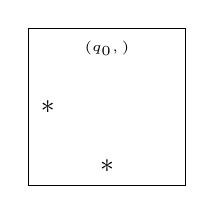
\begin{tikzpicture}
				\draw (-1,-1) -- (-1,1) -- (1,1) -- (1,-1) -- (-1,-1);
				\node at (0,.75) {\tiny$(q_0,\blank)$};
				\node at (.75, 0 ){\tiny$\blank$};
				\node at (0,-.75 ){$*$};
				\node at (-.75, 0 ){$*$};
			\end{tikzpicture}
		\caption{Initial tile}
		\end{subfigure}
	\begin{subfigure}{.5\textwidth}
					\centering
		\begin{tikzpicture}
			\draw (-1,-1) -- (-1,1) -- (1,1) -- (1,-1) -- (-1,-1);
			\node at (0,.75) {\tiny$\blank$};
			\node at (.75, 0 ){\tiny$\blank$};
			\node at (0,-.75 ){$*$};
			\node at (-.75, 0 ){\tiny$\blank$};
		\end{tikzpicture}
	\end{subfigure}
	\end{figure}
\item Tiles for simulating $R$ movement: For any transition $\delta(q,a) = (q', b, R)$ for $q\neq q_{acc}, q_{rej}$ we add $|\Gamma| + 1$ tiles
	\begin{figure}[H]
\begin{subfigure}{.5\textwidth}
			\centering
		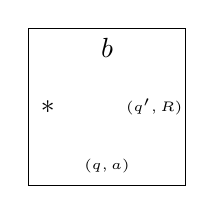
\begin{tikzpicture}
			\draw (-1,-1) -- (-1,1) -- (1,1) -- (1,-1) -- (-1,-1);
			\node at (0,.75) {$b$}; % Top
			\node at (.6, 0 ){\tiny$(q',R)$}; % right
			\node at (0,-.75 ){\tiny$(q,a)$}; %bottom
			\node at (-.75, 0 ){$*$}; %right
		\end{tikzpicture}
\end{subfigure}	
\begin{subfigure}{.5\textwidth}
	\centering
	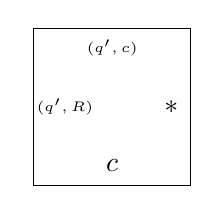
\begin{tikzpicture}
		\draw (-1,-1) -- (-1,1) -- (1,1) -- (1,-1) -- (-1,-1);
		\node at (0,.75) {\tiny$(q',c)$}; % Top
		\node at (-.6, 0 ){\tiny$(q',R)$}; % left
		\node at (0,-.75 ){$c$}; %bottom
		\node at (.75, 0 ){$*$}; %right
	\end{tikzpicture}
	\caption{for all $c\in \Gamma$}
\end{subfigure}	
\end{figure}
\item Tiles for simulating $L$ movement: For any transition $\delta(q,a) = (q', b, L)$ for $q\neq q_{acc}, q_{rej}$ we add $|\Gamma| + 1$ tiles
\begin{figure}[H]
	\begin{subfigure}{.5\textwidth}
		\centering
		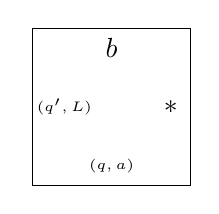
\begin{tikzpicture}
			\draw (-1,-1) -- (-1,1) -- (1,1) -- (1,-1) -- (-1,-1);
			\node at (0,.75) {$b$}; % Top
			\node at (-.6, 0 ){\tiny$(q',L)$}; % right
			\node at (0,-.75 ){\tiny$(q,a)$}; %bottom
			\node at (.75, 0 ){$*$}; %right
		\end{tikzpicture}
	\end{subfigure}	
	\begin{subfigure}{.5\textwidth}
		\centering
		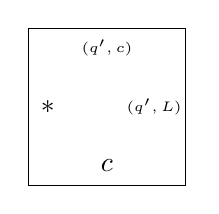
\begin{tikzpicture}
			\draw (-1,-1) -- (-1,1) -- (1,1) -- (1,-1) -- (-1,-1);
			\node at (0,.75) {\tiny$(q',c)$}; % Top
			\node at (.6, 0 ){\tiny$(q',L)$}; % right
			\node at (0,-.75 ){$c$}; %bottom
			\node at (-.75, 0 ){$*$}; %left
		\end{tikzpicture}
		\caption{for all $c\in \Gamma$}
	\end{subfigure}	
\end{figure}
\item Padding:
\begin{figure}[H]
	\centering
	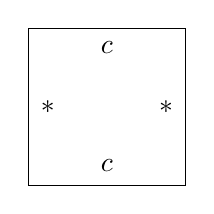
\begin{tikzpicture}
		\draw (-1,-1) -- (-1,1) -- (1,1) -- (1,-1) -- (-1,-1);
		\node at (0,.75) {$c$}; % Top
		\node at (.75, 0 ){$*$}; % right
		\node at (0,-.75 ){$c$}; %bottom
		\node at (-.75, 0 ){$*$}; %left
	\end{tikzpicture}
	\caption{for all $c\in \Gamma$}
\end{figure}
\end{itemize}
Note that this defines a mapping from TMs $\tbk{\Mm}$ into legal encodings of $TILE$. It is left to show that this is computable and that the reduction is correct:\\
For computability - given an encoding of $\delta$, there are finitely many tiles to encode - so this is computable.\\
For correctness - there exists an infinite tiling of our construction iff there is an inifnite sequence of configurations $C_0\ldots$ such that $C_i$ is written in the transition from row $i$ to row $i+1$, iff $C_0$ an initial configuration of $\Mm$ over $\varepsilon$ and $C_{i+1}$ is subsequent to $C_i$ iff $\Mm(\varepsilon)$ doesn't halt.
\end{proof}

\part{Complexity Theory} 
\chapter{Time Complexity}
\section{Measuring Complexity}
\begin{yellowBox}
	\begin{defn}[\TIME]
		For a function $t:\NN\to \NN$ we define
		\[
		\TIME(t(n)) = \cbk{\Ll\mid\text{ $\exists\Mm$ that decides $\Ll$ for $|w|=n$, halts after $O(t(n))$ steps}}
		\]
	\end{defn}
\end{yellowBox}
\begin{example}
	For $\Ll_{eq} = \{0^n1^n\}$ we saw $\Ll_{eq}\in \TIME(n^2)$. In fact - $\Ll_{eq} \in \TIME(n\log n)$\footnote{In every iteration - delete half of the $0$s and $1$s that survived until the current stage}.\\
	A TM with two strips can decide $\Ll_{eq}$ in $O(n)$ steps: Copy the $0$ prefix to the second strip and compare. Even though - $\Ll_{eq}\notin \TIME(n)$.\footnote{In fact - $\Ll\in \TIME(g(n))$ for $g\in o(n\log n)$ then $\Ll\in \Reg$. }
\end{example}
\begin{blueBox}
	\begin{thm}
		Let $t(n)$ be a function that satisfies $t(n) \geq n$\footnote{If $t(n)\leq n$ then we don't have time to read the input - so this is a reasonable assumption.}, then for any multi-strip TM that runs in $t(n)$ time, there is an equivalent single strip TM that runs in $t^2(n)$ time.
	\end{thm}
\end{blueBox}
\begin{proof}
	No Proof.
\end{proof}
\begin{blueBox}
	\begin{thm}
		If $t(n) \geq n$, and a nondeterministic TM that runs within $t(n)$ time, there is a deterministic single strip TM that runs within $2^{O(t(n))}$ time.
	\end{thm}
\end{blueBox}
\begin{yellowBox}
	\begin{defn}[Nondeterministic Complexity classes]
		Define:
		\begin{itemize}
			\item $\NTIME(t(n)) = \cbk{\Ll\mid\small\text{ $\exists\Mm$ nondeterministic decider that for $|w| = n|$ halts after $O(n)$ steps}}$
			\item $\PTIME = \displaystyle\bigcup_{k\geq 0}\TIME(n^k)$, with the petname $\P$.
			\item $\NPTIME = \displaystyle\bigcup_{k\geq 0}\NTIME(n^k)$, with the petname $\NP$.
			\item $\EXPTIME = \displaystyle\bigcup_{k\geq 0}\NTIME(2^{n^k})$
		\end{itemize}
	\end{defn}
\end{yellowBox}
\begin{blueBox}
	\begin{thm}
		$\P\subseteq\NP\subseteq\EXPTIME$
	\end{thm}
\end{blueBox}
\begin{proof}
	Any deterministic TM is a nondeterministic TM (first containment) and any nondeterministic TM can be simulated by a deterministic TM in exponential time (second containment).
\end{proof}
\section{The classes $\P,\NP$}
Consider two classical problems on graphs: Euler paths and Hamiltonian paths. Let $G = (V,E)$ (simple undirected graph). Let $\Gg_E, \Gg_H$ be the languages of graphs with Euler and Hamilton paths (respectively), then $\Gg_E\in \P$ (even $\NTIME(O(n))$). But we don't know $\Gg_H\nim{?}\in \P$. With that said - we do know $\Gg_H\in \NP$ by guessing a permutation of the vertices.
\begin{example}
	Define the language $$D-ST-HAMPATH = \cbk{\tbk{G,s,t}\mid \text{$G$ is a Directed graph with hamiltonian path }s\to t}$$
	For example - this digraph has an Hamiltonian $s\to t$ path:
	\begin{figure}[H]
		\centering
		\begin{tikzpicture}[shorten >=1pt,node distance=3cm,on grid,auto]
			\node[state] (s)   {$s$};
			\node[state] (q_1) at (2,2) {};
			\node[state] (q_2) at (2,-2) {};
			\node[state] (q_3) at (4,1) {};
			\node[state] (q_4) at (4,-1) {};
			\node[state] (q_5) at (6,2) {};
			\node[state] (q_6) at (6,-2) {};
			\node[state] (t) at (8,0) {$t$};
			
			
			\path[-stealth, thick]
			(s) edge [blue] (q_2)
			(q_1) edge (s) edge (q_2) edge [blue] (q_5)
			(q_2) edge [blue] (q_4) edge (q_6)
			(q_3) edge [blue] (q_1)
			(q_4) edge [blue] (q_3) edge (q_6)
			(q_5) edge [blue] (q_6) edge (t)
			(q_6) edge [blue] (t)
			
			;
		\end{tikzpicture}
		\caption{Graph with Hampath $s\to t$}
	\end{figure}
	\begin{prop}
		$D-ST-HAMPATH \in \EXPTIME$
	\end{prop}
\begin{proof}
	Given $G,s,t$, let $\pi_1\ldots \pi_{n!}$ denote the permutations of $V(G)$:
	\begin{enumerate}
		\item While $i\leq n!$:
		\item Let $\pi_i = v_1^i\ldots v_n^i$
		\item If $v_1^i = s, v_n^i = t$ and $(v_j^i,v_{j+1}^i)\in E$ - accept. Otherwise $i+=1$.
	\end{enumerate}
This algorithm runs in exponential time.
\end{proof}
Note that it is easy to check a given permutation. The reason that the algorithm is exponential is due to the number of possibilities.\\
Also - $D-ST-HAMPATH \in \NP$. Consider the NTM that guesses a permutation $\pi$ and checks if it is an $s,t$ Hamiltonian path.\\
What about $D-ST-HAMPATH^c$ (all graphs with no Hamiltonian path). Once again it is in $\EXPTIME$, but\footnote{Probably} not in $\NP$!
\end{example}
\begin{example}
	$COMPOSITE = \{x\mid x = p\cdot q\}$, of course $COMPOSITE^c = PRIME$. By assumption - $x$ is given in binary, so $COMPOSITE\in \NP$: Deciding prime numbers for an unary represented number is indeed polynomial. Since the input's length (in binary) is logarithmic in the unary representation - the time complexity is actually exponential in the representation.
\end{example}
\begin{yellowBox}
	\begin{defn}[Verifier]
		For a language $\Ll$, a TM $\Vv$ is a \textbf{Verifier} of $\Ll$ if\[
		\Ll = \cbk{w\mid \text{$\Vv$ accepts $\tbk{c,v}$ for some $x\in \Sigma^*$}}
		\]
		The verifier's complexity is measured WRT $|w|$: That is, runs in $poly(|w|)$ time on $\tbk{w,c}$. This implies $|c| = poly(|w|)$.
	\end{defn}
\end{yellowBox}
\begin{blueBox}
	\begin{thm}[Alternative characterization]
		$\Ll\in \NP \iff$ there exists a polynomial verifier for $\Ll$.
	\end{thm}
\end{blueBox}
\begin{proof}
	Assume $\Vv$ is a verifier. Construct a polynomial NTM that guesses a word $c$ with $|c| = poly(|w|)$ (all words with $|c| \leq f(|w|)$ where $f$ is $\Vv$'s time complexity) and runs $\Vv$ over $\tbk{w,c}$. For the other side - let $\Ll\in \NP$, then define $\Vv$ to accept $\tbk{w,c}\iff c$ is an accepting run of $\Mm_\Ll$ on $w$. Correctness is obvious, and since $\Mm_\Ll$ is polynomial - $|c| = poly(|w|)$, hence $\Vv$ is polynomial.
\end{proof}
\begin{example}
	A verifier for $D-ST-HAMPATH$ is the machine $\Vv$ with 
	\[
	\Ll(\Vv) = \cbk{\tbk{G,s,t,\pi}\mid \pi\text{ is a Hamiltonian $s,t$ path}}
	\]
\end{example}
\begin{example}
	A verifier for $COMPOSITE$:\[
	\Ll(\Vv) = \cbk{\tbk{x,p,q}\mid x = p\cdot q\quad q,p\neq 1}
	\]
	Of course there are variations and different verifiers (e.g - only one devisor)
\end{example}
\section{$\NP$-Completeness}
We would like to show that some things are not in $\P$. However - this is hard: We would need to prove that no polynomial TM decides the language. For this - we define a class of languages that had they been in $\P$, then things break beyond repair. For that - we need some more definitions. Until now (in computability theore) we used reductions to show that some problems are not in $\Rcr$, or not in $\RE$. Now we care about time complexity - so we need to take care of that.
\begin{yellowBox}
	\begin{defn}[Polynomialy Computable]
		A function $f:\Sigma^*\to \Sigma^*$ is said to be \textbf{Polyninomialy computable} if there is a polynomial TM $\Mm$ that computes it.
	\end{defn}
\begin{defn}
	[Polynomialy Reducable
	] We say $A$ is \textbf{Polynomialy Reducable} to $B$ (denote $A\leq_p B$) if there is a poly-computable function $f:\Sigma^*\to \Sigma^*$ with
	\[
	w\in A \iff f(w)\in B
	\]
\end{defn}
\end{yellowBox}
\begin{blueBox}
	\begin{thm}[Reduction Theorem]
		If $A\leq_p B$ and $B\in \P$ then $A\in \P$.
	\end{thm}
\end{blueBox}
\begin{proof}
	Let $\Mm_b$ poly TM for $B$ with complexity function $t_B$, and $f$ a poly-reduction $A\leq_p B$. A TM that decides $A$: Given $w$ compute $f(w)$ in $t_f(|w|)$ time, and $f(|w|)\leq t_f(w)$. Now run $\Mm_B$ over $f(w)$ in no more than $t_b(t_f(w))$ which is polynomial in $|w|$.
\end{proof}
With these definitions, we can define "hard languages":
\begin{yellowBox}
	\begin{defn}
		[$\NP $ - hard]We say that $\Ll$ is \textbf{$\NP$-Hard} if 
		\[
		\forall \Ll'\in \NP \quad \Ll'\leq_p \Ll
		\]
	\end{defn}
	\begin{defn}
		[$\NP $ - complete]We say that $\Ll$ is \textbf{$\NP$-Complete} if $\Ll\in \NP$ and is $\NP$-hard.\\
	\end{defn}
\end{yellowBox}
\begin{blueBox}
	\begin{thm}
		Let $\Ll\in \NP$. Then
		$\Ll\in \NPcomplete \iff$ there exists an $\NP$ hard language $\Ll'$ such that $\Ll'\leq_p \Ll$.
	\end{thm}
\end{blueBox}
\begin{proof}
	$\Leftarrow$ By transitivity. $\Rightarrow$ By reflexivity.
\end{proof}
\begin{example}
	define $SAT = \cbk{\tbk{\Theta}\mid \Theta\text{ is satisfyable}}\in \NP$ (by guessing an assignment). This language is $\NP$ complete - we will show this later.
\end{example}
\begin{yellowBox}
\begin{defn}
	[Conjunctive Normal Form] 
	A \textbf{literal} is a Boolean variable or a negated Boolean variable, as in $x$ or $\neg x$.
	A \textbf{Clause} is several literals connected with $\vee$s, as in ($x_1 \vee x_2\vee x_3 \vee \neg x_4$). A boolean formula is in \textbf{conjunctive normal form}, called a \textbf{cnf-formula}, if it comprises several clauses connected with $\wedge$s
\end{defn}
\end{yellowBox}
\begin{example}
	Let $3SAT = \cbk{\tbk{\varphi}\mid \varphi\in 3CNF}$\footnote{That is, $\varphi$ is in CNF form with $3$ literals in any clause.}\\
	Define $CLIQUE = \cbk{\tbk{G,k}\mid \text{The graph $G$ has a clique of size }k}$. We show $3SAT\leq_p CLIQUE$. It is easy to show that $3SAT\leq_m CLIQUE$: Given $\Theta$, check if it is satisfyable (in exponential time). If so - write $\tbk{K_2,2}$ on the strip. If not - write $\tbk{K_2,3}$.\\ 
	We now show a polynomial reduction $3SAT\leq_p CLIQUE$. Let $f:\varphi\mapsto \tbk{G,k}$ be the following function: Given 
	\[
	\varphi = \bigwedge_{i\in [m]}(\ell_i^1\vee \ell_i^2 \vee \ell_i^3)
	\]
	Define $G$ with $V(G) = \cbk{\ell_i^1,\ell_i^2,\ell_i^3\mid i\in [m]}$ (all the literals in $\varphi$), let $k = m$ (the number of clauses) and \[E(G) = V\times V\setminus \left(\cbk{(u,v)\mid u,v\text{ are in the same clause}}\cup \cbk{(u,v)\mid u = \neg v}\right)\]
	This build is polynomial- since there are $3m$ vertices and $O(m^2)$ edges. As for correctness, assume $\varphi$ is satisfyable and let $\nu:X\to \{T,F\}$ a satisfying valuation of $\varphi$. Thus, in any clause $C_j$ of $\varphi$ there is at least one literal $\ell^{k_j}_j$ with $\nu(\ell^{k_j}_j) = T$ (since it is in CNF). 
	\begin{prop}
		The collection $\cbk{\ell_j^{k_j}}_{j\in[m]}$ defines a clique in $G(\varphi)$
	\end{prop}
\begin{proof}
	Indeed, $(\ell^{k_{j}}_{j}, \ell^{k_i}_i)\in E$ since they are not from the same clause and cannot be negations of one another - since they are valued the same under $\nu$.
\end{proof}
Conversely, assume $G$ has a clique of size $m$. By definition of $E$, the clique contains exactly one representative of any clause $C_j$, and the representatives are consistent under valuations. This defines a satisfying valuation $\nu$ of $\varphi$ (exercise).\\

An example of this build is shown:
\begin{figure}[H]
	\centering
	\includegraphics[scale=.4]{3satReduction.jpg}
	\caption{The build from $\phi = (x_1\lor x_1 \lor \neg x_2)\land (\neg x_1 \lor \neg x_2\ \lor \neg x_2) \land (\neg x_1 \lor x_2 \lor x_2) $}
\end{figure}
\end{example}
\begin{blueBox}
	\begin{thm}
		$\Ll$ is $\NP$-complete $\Rightarrow$ $(\Ll\in \P\Rightarrow \P = \NP)$.
	\end{thm}
\end{blueBox}
\begin{proof}
	Let $\Ll$ an $\NP$-complete language. Hence, for any $\Ll'\in \NP$ there is a poly-reduction $f_{\Ll'}$ from $\Ll'$ to $\Ll$. Therefore $\Ll\in \P$ implies that $\Ll'\in \P$. Since $\P\subset \NP$ we get $\P = \NP$.
\end{proof}
\begin{example}
	Consider the language of vertex cover $VC = \cbk{\tbk{G,k}\mid G\text{ has a vertex cover of size at most }k}$. We show that this language is $\NP$-Complete.
	\begin{prop}
		$VC\in \NP$
	\end{prop}
\begin{proof}
	Consider the verifier that gets as input $\tbk{G,k,S}$ with $S\subset V$ and checks that $|S| \leq k$, then traverses $E$ and checks for $e\in E$ if there is a vertex $v\in V$ that is incident with $e$. If this holds for all $e\in E$, accept, otherwise reject. This is clearly correct. As for time complexity - checking the size of $S$ is at most $|V(G)|$. For any edge we compare it against all $V$, so total runtime of $O(|E|\cdot |V|)$, hence the runtime is $poly(\abs{\tbk{G}})$
\end{proof}
\begin{prop}
	$VC$ is $\NP$-hard.
\end{prop}
\begin{proof}
	We show that $CLIQUE \leq_p VC$, which results in $VC$ being $\NP$ hard. Consider $f:\tbk{G,k}\mapsto \tbk{G^c,n-k}$ with $G^c$ the complement graph of $G$. \\
	Assume $G$ has a clique of size $k$ and $v_1\ldots v_k$ clique vertices in $G$. No two of them are connected in $G^c$, then taking $S = V\setminus\{v_i\}_{i\in [k]}$ is hence a vertex cover of $G^c$, of size $n-k$. Conversely - if $G^c$ has a vertex cover of size $n-k$, denoted $S = \{v_1 \ldots v_{n - k}\}$, then all $V\setminus S$ define a clique: If $x,y\in V\setminus S$, we want to show $\{x,y\}\in E$, that is $\{x,y\}\notin E(G^c) = E^c$. If $\{x,y\}\in E^c$, since $x,y\notin S$ - $S$ is not a vertex cover of $G^c$, contradiction. Hence $V\setminus S$ defines a $k$-clique.
	As for time complexity - inverting the edges takes $O(|E|)$ time, and $k\mapsto n-k$ takes $O(|V|)$.
\end{proof}
\end{example}
\begin{yellowBox}
	\begin{defn}
		Given $G$, a dominating set $D\subset V$ is a set such that for all $v\in V $, $d(v,S) \leq 1$.
	\end{defn}
\end{yellowBox}
\begin{example}
	Consider $\cbk{\tbk{G,k}\mid \text{ There exists a dominating set in $G$ of size $k$}}$. We show that $DS$ is $\NP$ complete.\\
	A polynomial verifies would receive $\tbk{G,k,C}$ and checks that $C$ is a dominating set: Over $v\in V$ check if $v\in C$, if not - check if for any edge incident with $v$ if the other incident is in $C$. If exists - accept. Otherwise, reject. This is $poly(|G|)$: Iterating over $V$ is $O(|V|)$, over the edges is $O(|C|) = O(|V|)$, then total runtime of $O(|V|^2|E|)$.\\
	We reduce $VC\leq_p DS$. Consider the mapping $f: \tbk{G,k}\mapsto \tbk{G',k'}$: for $e = (x,y)\in E(G)$, $f$ adds a new vertex $v_e$ and the edges $\{(x,v_e), (y,v_e)\}$ (we only enrich the graph). Then $f$ returns $G'$ with $V(G') = V\cup \{v_e\}_{e\in E(G)}$ and $E(G') = E\cup \{(x,v_e), (y,v_e)\}_{e\in E(G)}$. Finally - $f$ counts the isolated nodes in $G$ (say, $m$) and returns $\tbk{G', k + m}$.\\
	Time complexity is $O(|V| + 3|E|) = O(V + |E|) = poly(|G|)$.\\
	As for correctness - assume $G$ has a VC $C$ of size $k$, and denote $F$ the isolated nodes of $G$: $C\cup F$ is a DS in $G'$ of size at most $k + m$: For $v\in V(G')$, it is either in $F$ (isolated), or not. If it is not, and $v\in V(G)$ - $v$ is in an edge $\{v,u\}$ and since $C$ is a VC of $G$, and $v$ is of distance $1$ to $C$. If $v = v_e$ for some $e$, then $e = \{x,y\}$, WLOG $x\in C$ and thus the distance to $C$ is at most $1$.\\
	
	Conversely - assume $G'$ has a dominating set of size $k'$ - it must contain the isolated vertices of $G$, discard them and we are left with a set $S$ of size $k$. If some $v_e\in S$, substitute it for some $x\in e = \{x,y\}$. This is a dominating set (proof omitted for I am awfully tired).
 \end{example}
\section{Cook - Levin Theorem}
\begin{blueBox}
	\begin{thm}[Cook - Levin Theorem]
		$3SAT\in \NPcomplete$.
	\end{thm}
\end{blueBox}
\begin{proof}
	First, $3SAT\in \NP$ by the verifier $\Vv$ with the language $\tbk{\varphi, \nu}$ where $\nu$ is a satisfying valuation of $\varphi$. It is left to show $3SAT\in \NPhard$.\\
	Let $\Ll\in \NP$. Define $f:w\mapsto \varphi\in 3CNF$. $\varphi$ is satisfyable if there exists a valuation, and $w\in \Ll$ if there exists an accepting run over $\Mm$ NTM that decides $\Ll$ within $t(|w|) = t(n) poly(n)$ time.. So we need to match runs to valuations of $\varphi$. That is - there exists a sequence of configurations $C_0\ldots C_m$ which is an accepting run of $\Mm$ over $w$, and $m = t(n)$. We build a matrix that in its entries there are characters from $S = \{\#\}\cup Q \cup \Gamma$:
	\begin{figure}[H]
		\centering
%		\includegraphics[scale=.5]{cooklevin.jpg}
		\caption{The tableux of configurations. We indexed from lower to upper, this is from the book.}
	\end{figure}
	The dimensions of this matrix is $t(n) \times  (t(n) + 3)$ (at most). The formula $\varphi$ will say "there exists such matrix of an accepting run". Let us construct it:\\
	Its variables are:
	\begin{align*}
		\forall i,j \text{ entry in the matrix, and } s\in S \text{ - assign a variable } x_{i,j,s}\text{ that describes }A^j_i = s
	\end{align*}
	$\varphi = \phi_{cell}\land \phi_{init} \land \phi_{acc} \land \phi$ With:
	\begin{itemize}
		\item $\phi_{cell}$ says "a satisfying valuation describes an accepting run" (that is, no $\nu(x_{1,1,a}) = \nu(x_{1,1,b})$)
		\item $\phi_{init}$ says "an assignment to the first row complies with the initial configuration of $\Mm$ over $w$".
		\item $\phi_{acc}$ says "there is a row that describes an accepting configuration".
		\item $\phi_{move}$ says "ascending in the matrix complies with transition between subsequent configurations".
	\end{itemize}
So:
\begin{align*}
		&\phi_{cell} = \bigwedge_{i,j}\left[\overbrace{\left(\bigvee_{s\in S} x_{i,j,s}\right)}^{\text{Every cell contains a letter}}\land \overbrace{\left(\bigwedge_{s_1\neq s_2} \neg x_{i,j,s_1}\lor \neg x_{i,j,s_2}\right)}^\text{Only one letter}\right]\\
		&\varphi_{init} =\overbrace{ x_{1,1,\#}\land x_{2,1,q_0}\land x_{3,1,w_1}\land\ldots x_{n+2,n,w_n}\land x_{n+3,1,\blank},\ldots\land x_{t(n) + 3, 1, \#}}^{\text{The first row is the initial configuratoin}}\\
		& \varphi_{acc} =\overbrace{ \bigvee_{j\in [t(n)]}\left[\bigvee_{2\leq i\leq t(n) + 2} x_{i,j,q_{acc}}\right]}^{\text{In some row there is $q_{acc}$}}\\
\end{align*}
For $\phi_{move}$ - it is sufficient to check submatrices of size $3\times 2$ (since legal transitions are very local). That is - there is a set $W$ of finite cardinality  of legal "windows" (submatrices) of size $3\times 2$. $\phi_{move}$ will say "all windows of size $3\times 2$ are from $W$":
\[
\phi_{move} = \bigwedge_{\underset{i\leq t(n) + 1}{j\leq t(n) - 1}}
\left[\bigvee_{(s_1,s_2,s_3,s_4,s_5,s_6)\in W}\overbrace{x_{i,j,s_1} \land x_{i+1,j, s_2}\land x_{i+2, j ,s_2}\land x_{i, j+1, s_4}\land x_{i+1, j+1, s_5}\land x_{i+2, j+1, s_6}}^{\text{the window is legal}} \right]
\]
We now define $W$ (and that it is of polynomial size in $n$). For any transition $\delta(q_1,a)\ni \tbk{q_2, b,R}$ (and of course similarly for $L$), add windows of the following types:\\
\begin{figure}[H]
	\centering
	\includegraphics[scale=0.5]{cooklevinwindows.jpg}
	\caption{Examples of legal windows}
\end{figure}
And in sequential notation (for example) - $(q_1, a, c, b, q_2, b)$. So for any transition there is a finite number of valid windows. In fact - this is independent of $|w|$ - so we're all good.\\
We show that $\varphi$ is satisfyable iff there is an accepting run of $\Mm$ over $w$: Assume $f$ is a truthful valuation of $\phi$, then $f$ describes a matrix of size $(t(n) +3 )\times t(n)$. Since $\phi_{init}$ is satisfied - the first row describes the initial configuration of $\Mm$ on $w$. Since $\phi_{move}$ is satisfied - the $j+1$'s row is a subsequent configuration of the $j$'s row. Since $\phi_{acc}$ is satisfied - at some point, we reach an accepting configuration. Therefore - there is an accepting run of $\Mm$ on $w$.\\
Conversely - if there exists an accepting run of $\Mm$ over $w$, there is a matrix with the sequence of configuration describing a satisfying valuation of $\phi$.\\

All constructions are polynomial in $t(n)$, hence polynomial in $n$ - so the reduction is polynomial.\\

$\phi$ is in $CNF$ form, but not $3CNF$. We will show in the exercise that we can reform a formula in $CNF$ to a formula in $3CNF$ in polynomial time.
\end{proof}
\section{More examples}
As we defined $\NP$ hardness and $\NP$ completeness, there are symmetric definitions for $\coNP$ (as well as for any complexity class). We see some examples:
\begin{example}
	Define $VAL = \cbk{\tbk{\phi}\mid \text{All valuations satisfy $\phi$}}$. That is, for any $\nu:X\to \{T,F\}$ we have $\nu \vDash \phi$, iff there is no $\nu$ with $\nu \vDash \neg \varphi$ iff $\phi\notin SAT$. So $VAL\in \coNP$
\end{example}
\begin{blueBox}
	\begin{thm}
		$\Ll$ is $\coNP$-complete $\iff$ $\Ll^c$ is $\NP$-complete.
	\end{thm}
\end{blueBox}
\begin{proof}
	By definition, for any $\Ll'\in \coNP$ we have $\Ll'^c\in \NP$. Therefore there is a reduction $\Ll'^c\leq_p \Ll^c$ since $\Ll^c$ is $\NP$-hard. The same reduction implies $\Ll'\leq_p \Ll$, hence $\Ll$ is $\coNP$ hard.
\end{proof}
\subsection*{Another reduction $3SAT\leq_p CLIQUE$}
Given $\phi = {\displaystyle \bigwedge_{i\leq j\leq m}}\left(\ell^1_j \lor \ell^2_j \lor \ell^3_j\right)$, we would like to define an undirected graph $G$ and a number $k$ such that $K_k\subset G$ iff $\phi$ is satisfyable. Consider the clause $C_j = x_1\lor \neg x_2 \lor x_3$. There are $2^3-1$ satisfying valuations\footnote{Consider the equivalent disjunctive form of the clause}. We will consider these valuations as \textbf{restrictions}. Denote $F_j = \{\nu^l_j\}_{l\in [7]}$ the satisfying valuations of $C_j$ (over its three variables). Define $V(G) = {\displaystyle \bigcup_{j\in [m]} F_j}$.\\
\textbf{I can't find the example in my photos - If anyone could send it to me, that'd be great }\\
And let $E(G)$ be the set of edges with no "contradiction", that is $\{\nu^{l_1}_j,\nu^{l_2}_t\}\in E(G)$ agree on their common variables (and of course no loops). We claim $K_m\subset G$ iff there is a satisfying valuation.\\
Note that this construction is polynomial in $|\phi|$ - since there are at most $8\cdot m$ valuations to check (to defnie nodes), and the edges need at most $O(3\cdot m^2)$ things to check.
\begin{remark}
	This construction is exponential in $3$ - that is, for a fixed $k$, this will work for any $k-CNF$ class of formulas.
\end{remark}
\chapter{Space Complexity}
\section{Introduction}
\begin{yellowBox}
	\begin{defn}[Space Complexity]
		We say that a (single strip) TM $\Mm$ works in \textbf{Space Complexity} $S:\NN\to \NN$ if for any input $w$, $\Mm$ uses at most $S(|w|)$ cells of the strip.
	\end{defn}
\end{yellowBox}
As in time complexity - there are space complexity classes.
\begin{yellowBox}
	\begin{defn}
		Given $S:\NN\to \NN$, we define $$\SPACE(S(n)) = \tbk{\Ll\mid \Ll\text{ is decided by a TM with space compexity } O(S(n))}$$
	\end{defn}
\end{yellowBox}
\begin{blueBox}
	\begin{thm}
		$TIME(f(n))\subset \SPACE(f(n))$
	\end{thm}
\end{blueBox}
\begin{proof}
	If a TM works in time $f(n)$, it can reach with its head only to $f(n)$ cells.
\end{proof}
\begin{blueBox}
	\begin{thm}
		$\SPACE(f(n))\subset \TIME(2^{O(f(n))})$
	\end{thm}
\end{blueBox}
\begin{proof}
	We compute how many configurations exists to a TM $\Mm$ with space complexity $S(n)$: $|Q|\cdot S(n) \cdot |\Gamma|^{S(n)} = c_1 \cdot S(n) \cdot c_2^{S(n)} = 2^{O(S(n))}$.\\
	Since $\Mm$ decides a language and is deterministic, it does not repeat the same configuration twice. Therefore - it halts within $2^{O(S(n))}$ steps.
\end{proof}
\section{Space Complexity Classes}
\begin{yellowBox}
	\begin{defn}
		We define, similarly to time complexity classes:
		\begin{itemize}
			\item $\NSPACE(S(n)) = \cbk{\Ll\mid \text{$\Ll$ i decided by a nondeterministic TM with $O(S(n)$ space)}}$
			\item $\PSPACE = {\displaystyle \bigcup_{k\in \NN}\SPACE(n^k)}$
			\item $\NPSPACE = {\displaystyle \bigcup_{k\in \NN}\NSPACE(n^k)}$
		\end{itemize}
	\end{defn}
\end{yellowBox}
\begin{remark}
	By the previous theorems, we know:
	\[PTIMES\subset \PSPACE\qquad \PSPACE\subset EXPTIME\]
\end{remark}
\begin{example}
	$SAT\in \PSPACE$. The idea is to check all valuations of a given formula (by using the same space) one after the other (time-wise). Let $\nu_1\ldots \nu_{2^n}$ an ordering of the valuations (of $\phi$ with $n$ variables), such that given $\nu_i$, we can find $\nu_{i+1}$ with linear space - or return $\perp$ if we are in the last valuations (eg - lexicographic order). $\Mm$ operates the following way: One strip will hold $\nu_1$, the other the value $\nu(\varphi)$. While the first strip does not say $\perp$, $\Mm$ computes $\nu_i(\varphi)$. If $T$ -halt and accept. Otherwise - update in the first strip to the valuation $\nu_{i+1}$. When the first strip contains $\perp$ - reject.\\
	
	Note that the first strip requires $O(n)$ cells (and the space required for an update). The second strip needs $O(|\phi|)$ cells for computing $\nu(\phi)$.
	\end{example}
This can easily be extended for any language in $\NP$.
\begin{blueBox}
\begin{thm}
	$\NP\subset \PSPACE$
\end{thm}
\end{blueBox}
\begin{proof}
	Let $\Ll\in \NP$, ad let $\Vv$ be a polynomial verifier of $\Ll$, with $f:\NN\to \NN$ bounding  $\Vv$'s runtime. Let $c_1\ldots c_{|\Sigma|^{f(|w|)}}$ the lexicographic ordering of $\Sigma^{\leq f(|w|)}$. A TM that decides $\Ll$ in polyspace would go over all $c_i$ (the "witnesses") and simulate $\Vv$ to check them. The details can be completed as in the previous example.
\end{proof}
\begin{example}
	Denote $EMPTY_{NFA} = \cbk{\tbk{\Aa}\mid \Ll(\Aa) = \emptyset}$ and $ALL_{NFA} = \cbk{\tbk{\Aa}\mid \Ll(\Aa) = \Sigma^*}$ and consider their complements $\overline{EMPTY_{NFA}}, \overline{ALL_{NFA}}$. It is clear that $\overline{EMPTY_{NFA}}\in \NP$ - by the witness in the form of a word (of length corresponding to a simple path over $\Aa$'s graph, therefore polynomial in $\tbk{\Aa}$). We need to show that it can be verified in polytime (since $\Aa$ is nondeterministic it is not trivial). Consider the automaton $\Aa_w$  with $\Ll(\Aa_w) = \{w\}$. Then the product automaton $\Aa\times \Aa_w$\footnote{A variation of this} has the language $\Ll(\Aa)\cap \Ll(\Aa_w)$. So $w\in \Ll(\Aa)$ iff $\Ll(\Aa\times \Aa_w)\neq \emptyset$. Checking this is in fact checking if an accepting state is reachable from some initial state. In Algorithms course we saw that this is polynomial in the graph's size.\\
	
	For $\overline{ALL_{NFA}}$, how would we go about that? For $\overline{ALL_{DFA}}$ this is easy (since the complement automaton would have empty language). It is not clear that $\overline{ALL_{NFA}}\in \NP$. We will construct NFA $\Aa$ with $\Ll(\Aa)\neq \Sigma^*$, but the shortest word $\Aa$ rejects is exponential in $|\Aa|$:\\
	Let $i\geq 1$, consider the first $i$ prime numbers $p_1\ldots p_i$, and consider the language: $$\Ll_i = \cbk{w\mid |w| \text{ is not divisible by one of $p_1 \ldots p_i$}}$$
	Denote $\Aa_{p_j}$ the automaton with a cycle of size $p_j$ and the first state rejects. Then $\Aa_i = {\displaystyle \bigsqcup_{j\in [i]} A_{p_j}}$, and since $|p_j| = O(j\log j)$, $|\Aa_i|$ is polynomial in $i$. Consider $w^* = a^{\prod_{j\in i}p_j}$, then $w^*\notin \Ll_i$, but $|w^*| \geq 2^i= \exp(i)$. Then there is a word which is not in $\Ll_i = \Ll(\Aa_i)$. We need to show that $a^y$ with $y<\prod_{j\in i}p_j$ is accepted. This is because when we decompose $y$ into prime components, there must appear a component which is not in $\{p_j\}_{j\in [i]}$.
\end{example}
\begin{claim}
	$\overline{ALL_{NFA}}\in \NPSPACE$.
\end{claim}
\begin{proof}
	Given $\Aa$ NFA, the following are equivalent:
	\begin{enumerate}
		\item $\Ll(\Aa)\neq \Sigma^*$
		\item $\Ll(\overline{\Dd}) \neq \emptyset$\footnote{The accepting states of $\overline{\Dd}$ are exactly $S\subset Q$ such that $S\cap F = \emptyset$} with $\Dd$ the $DFA$ generated by the subset construction over $\Aa$.
		\item There exists an increasing sequence of states $\{Q_i\}_{i=0}^k$ with $k\leq 2^{|Q|}$ such that $Q_0$ is the set of initial states of $\Aa$, and for all $i$, $Q_{i+1} = \delta(Q_i, \sigma_i)$ for some $\sigma$, and $Q_k\cap F = \emptyset$ (that is, this is a sequence corresponding to an accepting run of some word in $\overline{\Dd}$).
	\end{enumerate}
	$(1\iff 2)$ Since $\Ll(\overline{\Dd}) = \Sigma^\setminus \Ll(\Aa)$, this is immediate.\\
	$(2\iff 3)$ $\Ll(\overline{\Dd})\neq \emptyset \iff$ there is a word with length $\leq 2^{|Q|}$ (number of states of $\overline{\Dd}$) that is accepted (because there is a word that's accepted over a simple path) $\iff$ there exists the required sequence.\\
	
	Then define an NTM operating in polyspace $\Mm$ and decides $\overline{ALL_{NFA}}$: On the strip we will hold a counter (until $2^{|Q|}$, requires $O(|Q|)$ space!) and the encoding of the current state $S = Q_{i}$ (an instance of a subset of $Q$, lets say represented by a subset of $[n]$ - still polyspace in $|Q|$)
	\begin{enumerate}
		\item Write $Q_0$ on the strip (where we keep states)
		\item writes $i=0$ (where we keep counter)
		\item While $i\leq 2^{|Q|}$:
		\begin{enumerate}[3.1]
			\item If $Q_i \cap F = \emptyset$ - halt and accept
			\item Otherwise - \textbf{guess} a letter $\sigma\in \Sigma$ and updates the strips: $Q_i$ is substituted with $\delta(Q_i, \sigma)$ and $i++$.
		\end{enumerate}
	\item Halt and reject
	\end{enumerate}
\end{proof}
\begin{blueBox}
	\begin{thm}[Savitch Theorem]
		For any space complexity $S$ with $S(n) \geq n$, \[\NSPACE(S(n)) \subset \SPACE(S^2(n))\]
	\end{thm}
\end{blueBox}
\begin{proof}
	Let $\Nn\in \NSPACE(S(n))$. Preliminaries: 
	\begin{itemize}
		\item For any $w$, $\Nn$ has a unique initial configuration $C_{init}^w$.
		\item $\Nn$ has a unique accepting configuration (say, when $\Mm$ arrives at an accepting configuration - it cleans the strip and goes back to the beginning of the strip), denoted $C_{acc}$.
		\item Let $d$ be such that $\Nn$ has at most $2^{d\cdot S(n)}$ different configurations during a run over a word of length $n$.
	\end{itemize} 
We build a deterministic procedure\footnote{A part of a TM, we will iteratively run this procedure} $\Mm = reach(C_1, C_2, t)$ that decides if the configuration $C_2$ is reachable from $C_1$ within $t$ steps. Its space complexity would be $O(\log(t) + S(n))\cdot \log(t)$. Then given $w$, an NTM $\Mm'$ would check $reach(C_{init}^w, C_{acc}, 2^{d\cdot S(|w|)})$. Note that indeed $\Mm$ accepts $w$ iff $reach(C_{init}^w, C_{acc}, 2^{d\cdot S(|w|)})$, and that the space complexity would be $O(S^2(n))$.\\

The procedure:
\begin{enumerate}
	\item If $C_1 = C_2$ or $C_2$ is subsequent of $C_1$ - accept.
	\item Otherwise - Iterate over all configurations $C$ that use $S(|w|)$ cells. For each of them:
	\begin{enumerate}[2.1]
		\item Check if $reach(C_1, C, \lceil\frac{t}{2}\rceil)$
		\item Check if $reach(C, C_2, \lfloor\frac{t}{2}\rfloor)$
		\item If both accepted - accept.
	\end{enumerate}
\item Reject
\end{enumerate}
Correctness is obvious. The hard part is checking the space complexity. The recursion's depth is $log(t)$. The recursion "saves" only one branch of the recursion tree in any given moment. Hence we save only the path from the root to the current node, and information related to iterating over all configurations. That is - to save a single node, we need:
\[2\cdot S(n) + \log(t)\]
space to save any node (two configurations $S(n)$ and current path length $\log(t)$), information to iterate over configurations is $S(n)$, so total space complexity $O(S(n) + \log(t))\cdot \log(t)$.\\
How does $reach$ "knows" $S(n)$? If $S(n)$ is known - everything's fine. If $S(n)$ is unknown, build the same TM with a twist. Note that $reach$ can be used to check if there exists a reachable configuration that uses $i$ cells: Iterate over all configurations that uses $i$ cells, and for each such $C$, check $reach(C_{init}^w, C, 2^{di})$ (assuming $S(n) = i$). We build an outer loop to deterministically decide if $\Mm$ accepts $w$:
\begin{enumerate}
	\item For $i\in \NN$:
	\begin{enumerate}
		\item Check if there is a reachable configuration that uses $i$ cells? If not - reject
		\item If there is - run the previously built $\Mm$ with $S(n) = i$. If accepted - accept. Otherwise, $i++$.
	\end{enumerate}
\end{enumerate}
\end{proof}

\begin{cor}
	$$\NPSPACE = \PSPACE = \coNPSPACE = \coPSPACE$$
\end{cor}

\section{Space-Hardness and Space-Completeness}
\begin{yellowBox}
	\begin{defn}[$\PSPACE$-hard]
		We say that $\Ll$ is \textbf{$\PSPACE$-hard} if for any $\Ll'\in \PSPACE$, $\Ll'\leq_p \Ll$. 
	\end{defn}
\begin{remark}
	The same notation of $\leq_p$ as in time complexity.
\end{remark}
	\begin{defn}[$\PSPACE$ - complete]
		We say that $\Ll$ is \textbf{$\PSPACE$-complete} if $\Ll\in \PSPACE$ and is $\PSPACE$-hard.
	\end{defn}
\end{yellowBox}
We will see a $\PSPACE$-complete language. For this we need a new definition regarding boolean formulas:
\begin{yellowBox}
	\begin{defn}
		We say a formula $\phi$ is \textbf{Fully Quantified} if any variable $x\in \phi$ is connected to a quantifier $\exists, \forall$
	\end{defn}
\end{yellowBox}
\begin{example}
	Define $TQBF = \cbk{\tbk{\phi}\mid \phi\text{ is a True fully quantifid formula}}$. That is, $\phi\in TQBF$ is a totally quantified tautology.
	\begin{claim}
		$TQBF\in \PSPACE$
	\end{claim}
\begin{proof}
	Define $\Mm$ to operate recursively over $\phi$:\begin{enumerate}
		\item (Base Case) If $\phi$ is without quantifier, then $\Mm$ valuates $\phi$ and accepts if True. Otherwise - reject.
		\item If $\phi = (\exists x) \psi$, then run $\Mm(\psi)$ recursively twice: once with $x = 0$ and once with $x=1$. Accept if one of them accepts - accept. Otherwise reject.
		\item If $\phi = \forall x \psi$ then run $\Mm(\psi)$ recursively with $x=0$ and with $x=1$. Accept if both accepted. Otherwise reject.
	\end{enumerate}
This obviously decides $TQBF$. Note that the depth of enery branch in the recursion tree is bounded by number of variables of $\phi$ $\leq |\phi|$, and for any variable we run at most twice. In every stage we remember which variables were substituted and what's left to check - $O(|\phi|)$ space. Finally, in the base case we valuate $\phi$ which takes $O(|\phi|)$ space - all in all, the space complexity is $O(|\phi|^2)$ - as required.
\end{proof}
We would like not wo show it is complete in $\PSPACE$. How do we encode configurations using boolean formulas?\\
Let $\Mm$ be a TM and assume $\Mm$ uses $S$ strip cells. Encode the following way:
\begin{enumerate}
	\item For $i\in [S]$ define a variable $x_{ia}$ which encodes "$a$" is written in cell $i$".
	\item For $i\in [S]$ define a variable $y_i$ which encodes "The reading head is over cell $i$"
	\item For any $q\in Q$ define a variable $z_q$ which encodes "The machine $\Mm$ is in state $q$".
\end{enumerate}
\begin{blueBox}
	\begin{thm}
		Let $\Mm$ be a TM. Then:
		\begin{enumerate}
			\item There exists a formula $\phi_{valid}(C)$ which is True iff $C$ is a valid encoding of a configuration of $\Mm$.
			\item There exists a formula $\phi(C_1,C_2)$ which is True iff $C_2$ is subsequent of $C_1$.
		\end{enumerate}
	In addition - both formulas are computable in polyspace in $S$.
	\end{thm}
\end{blueBox}
\begin{proof}
	Define:
	\[
	\phi_{valid}(C) = \bigwedge_{i\in [S]}\bigvee_{a\in \Gamma}\left(x_{ia}\land \bigwedge_{b\in \Gamma\setminus\{a\}}\neg x_{ib}\right)\land\bigvee_{i\in [S]}\left(y_i\land \bigwedge_{j\in [S]\setminus \{i\}}\neg y_j\right)\land\bigvee_{q\in Q}\left(z_q\land \bigwedge_{q'\in Q\setminus\{q\}}z_{q'}\right)
	\]
	Note that $|\phi_{valid}(C) = O(S^2)$. Now define for any $i\in [S], a\in \Gamma, q\in Q$, if $\delta(q,a) = (r,b,R)$ then define:
	\[
	\psi_{iaq}(C_1,C_2) = (x^1_{ia}\land y^1_i\land z^1_q)\Rightarrow (x^2_{i,b}\land y^2_{i+1}\land z_r\bigwedge_{j\in [S]\setminus \{i\}}\bigwedge_{d\in \Gamma}(x^1_{jd}\iff x^2_{jd}))
	\]
	And of course, symmetrically define for transition to $L$, and for exceptions (e.g - when we are in cell $1$ and move to the left).
	Convince yourself that this actually encodes the transition. Now define:
	\[
	\phi(C_1, C_2) = \phi_{valid}(C_1)\land \phi_{valid}(C_2) \land \bigwedge_{i\in [S]}\bigwedge_{a\in \Gamma}\bigwedge_{q\in Q}\psi_{iaq}(C_1,C_2)
	\]
	Once again - the length of $\psi(C_1, C_2) = O(S^2)$
\end{proof}
\begin{claim}
	$TQBF$ is $\PSPACE$-hard.
\end{claim}
\begin{proof}
	Let $\Ll\in \PSPACE$ be a language. We would like to build a function $f:w\mapsto\phi_{w}$ such that $w\in \Ll\iff \phi_w\in TQBF$. Let $\Mm$ be a TM that decides $\Ll$ is polyspace. \\
	Define a formula that says "$C_2$ is reachable from $C_1$ within $k$ steps": 
	\[
	\phi_k(C_1,C_2) = \exists C_m\forall C_3,C_4\left[(C_3 = C_1)\land (C_4 = C_m)\lor (C_3=C_m)\land(C_4 = C_2)\right]\Rightarrow \phi_{k/2}(C_3,C_4)
	\]
	Any recursive call is polynomial and there is only one branch - so no exponential number of leaves. This formula is built in polyspace in $w$.
\end{proof}
\end{example}
\begin{example}
	Consider the language $\overline{ALL_{NFA}}$. We've shown that $\overline{ALL_{NFA}}\in \NPSPACE$. By Savitch - $\overline{ALL_{NFA}}, ALL_{NFA}\in \PSPACE$. We will see that $\overline{ALL_{NFA}}$ is $\PSPACE$-hard.
\end{example}
\section{Sublinear Space Complexity}
\begin{yellowBox}
	\begin{defn}
		Define $$LOGSPACE = \SPACE(\log(n)), NLOGSPACE =\NSPACE(\log(n))$$ denoted $L,NL$ respectively.
	\end{defn}
\begin{remark}
	Since the input itself takes $|w|$ space, we change the computational model a little: We require two strips, and that the work strip would be of logarithmic space.
\end{remark}
\end{yellowBox}
\begin{example}
	Let $EQ = \{0^k1^k\mid k\in NN_0\}$. We saw that $EQ\in \P$, but the algorithm wrote on all of the cells, thus $EQ\in \SPACE(n)$. We define a TM $\Mm$ that decides $EQ$ in $LOGSPACE$. The machine maintains two counters $C_0, C_1$ in binary, and counts. each counter takes $O(\log(n))$ cells. Then compares them.
\end{example}
\begin{example}
	Recall $PATH = \cbk{\tbk{G,s,t}\mid G\text{ is a directed graph and there is a path }s\to t}\in \P$. We show $PATH\in NLOGSPACE$ by guessing a path. We only need to "remember" on which node we stand in any given moment moment. We also maintain a counter $i$ until $|V|$ (once again, in binary). $\Mm$ operates the following way:
	\begin{enumerate}
		\item Write on the strip $s_0 = s, i=0$.
		\item While $i\leq |V|$, if $s_i = t$ then halt and accept. Otherwise - guess a neighbor $s_i\to s_{i+1}$, and $i++$.  
		\item Halt and reject.
	\end{enumerate}
Correctness is clear: There is a path $s\to t$ iff there is a simple path $s\to t$ iff $\Mm$ might guess this path iff $\Mm$ accepts.\\

Is $PATH\in LOGSPACE$? By Savitch. $\NSPACE(s(n))\subset \SPACE(s^2(n))$, but this does not imply $NLOGSPACE\subset LOGSPACE$
\end{example}
\subsection*{Completeness and Hardness}
The definitions are the same - with a twist: Polynomial reductions are not good enough\footnote{We will see that $NL\subset \PTIME$} - so we need a new notion of reduction:
\begin{yellowBox}
	\begin{defn}[Logspace Reduction]
		A function $f:\Sigma^*\to \Sigma^*$ is a \textbf{Logspace Reduction} if there exists a \textbf{Logspace transducer} $\Mm$. That is, $f$ is computable by $\Mm$ which operates with $3$ strips (input - RO, work - RW, and output - WO): The work strip is with $O(\log(|w|)$ cells, and $\Mm$ writes $f(w)$ on the output strip.
	\end{defn}
\begin{remark}
	If $f$ is such that $w\in \Aa \iff f(w)\in \Bb$, we write $\Aa\leq_L \Bb$.
\end{remark}
\end{yellowBox}
\begin{example}
	Consider a digraph with two types of nodes. An initial node $s$ holds a token. The first type node ("first player") does not want the token to reach $t$, and the second type node ("second player") wants the token to reach $t$. This problem is in $\P$ and in fact is $\P$-complete.
\end{example}
\begin{blueBox}
	\begin{thm}
		$PATH$ is $NL$-complete.
	\end{thm}
\end{blueBox}
\begin{proof}
	It is left to show that for any $\Ll\in NL$, $\Ll\leq_L PATH$. The idea: let $\Mm$ be a logspace decider of $\Ll$. The graph $G$ would be the configurations graph, $s=  C^w_{init}$ and $t = C_{acc}$ the accepting configuration (as always, assume uniqueness). $G$'s nodes would be all configurations, and edges iff subsequent configurations.\\
	Any configuration is described by an element of $\Gamma^i (\Gamma\times Q)\Gamma^{s(n) - i+1}\# (0+1)^{\log(n)}$, which requires $2\log(n) + 1 = O(\log(n))$ space. The reduction go over all words over $\Gamma\cup (Q\times \Gamma)\cup \{\#,0,1\}$ and write those who describe a valid configuration. These are $V(G)$. For $E$, iterate over pairs of words and copy those who correspond to subsequent configurations. For $s,t$ - we just write them down, as we know their structure.
\end{proof}
\begin{remark}
	There were some results for which we demanded $s(n) \geq n$. This is because we bounded the number of configurations with $2^{ds(n)}$ for some $d$, and wanted to notice something exponential. Even when $s(n) = O(\log(n))$, there exists $d$ such that the number of configurations is bounded by $2^{d\cdot s(n)}$: In this case, the number of configurations is $|Q|\cdot |\Gamma|^{s(n)}\cdot s(n)\cdot n$ with the $n$ indicating the reading head's location in the input strip. When $s(n) = O(\log(n))$, the number of configurations is bounded by $k_1\cdot k_2^{d_1 \log(n)}(d_1\log(n))2^{\log(n)}\leq 2^{d\log(n)}$ for some $d$. Hence Savich holds even in logspace.
\end{remark}
\begin{blueBox}
	\begin{thm}
		$NL\subset \P$
	\end{thm}
\end{blueBox}
\begin{proof}
	Let $\Ll\in NL$. Reduce $\Ll\leq_L PATH$ (takes polytime since the number of configurations of $\Ll$ is polynomial). Afterwards run $DFS$ or $BFS$ (in polytime) and respond accordingly.
\end{proof}


\end{document}

